\documentclass{article}
\usepackage[utf8]{inputenc}

\usepackage{float}
\usepackage{newfloat}
\DeclareFloatingEnvironment[
    fileext=los,
    listname=List of Figures,
    name=Figure,
    placement=H,
    within=section,
]{scheme}

\usepackage{adjustbox}
\usepackage{algorithm}
\usepackage{algpseudocode}
\usepackage{amsfonts}
\usepackage{amsmath}
\usepackage{physics}
\usepackage{tikz}
\usepackage{mathdots}
\usepackage{yhmath}
\usepackage{cancel}
\usepackage{color}
\usepackage{siunitx}
\usepackage{array}
\usepackage{multirow}
\usepackage{amssymb}
\usepackage{gensymb}
\usepackage{tabularx}
\usepackage{extarrows}
\usepackage{booktabs}
\usepackage{biblatex}
\addbibresource{sample.bib}
\usetikzlibrary{fadings}
\usetikzlibrary{patterns}
\usetikzlibrary{shadows.blur}
\usetikzlibrary{shapes}
\usepackage{hyperref}


\title{Key Evolving Signature Scheme - Formal Specification}
\author{Aaron Schutza }
\date{October 2021}

\begin{document}

\maketitle

\section{Introduction}
This document specifies a protocol for deriving keys that are securely erased as they are used to construct proofs that authenticate with succinct verification information with the intent to aid implementers. Key Evolving Signature (KES) schemes generate a time series of public-private key-pairs in an ordered derivation process where a parent key derives the child key in a trapdoor operation.  The parent key must be non-recoverable from the child key to ensure past signatures cannot be reforged.  The KES public-private keys considered here are designed for use in the individual rounds in a blockchain protocol to sign block headers.  We propose coupling a simplified linear-secret-key scheme first put forth by Anderson \cite{Anderson1997}, Bellare, and Miner \cite{BM1999} with the MMM construction \cite{MMM}. The goal is to retain a high number of time steps per registration, while having the shortest signature size possible.  The linear-secret-key composition enables a high number of time steps while retaining succinct proofs with the tradeoff being that the secret key becomes large.  This construction is designed for use with round based proof-of-stake blockchain protocols where forward security is required and succinct signatures and public keys are desired.  We realize this construction with an Ed25519 signing routine \cite{ed25519}, and an evolving key and accumulator scheme that builds on the product composition from the MMM construction \cite{MMM}.  Finally the format of public-private keys and certificates in this KES construction is specified with test vectors.

\section{Motivation}
 The use of a key evolving scheme is crucial for forward security of a proof-of-stake platform that does not have a checkpoint mechanism.  
 The KES portion of this functionality prevents long range attacks in an environment where node operators may be coerced to reveal old private staking information.  
 Secure erasure is performed in the KES setup and erases the key required to sign in a given time step. 
 This means that honest activity will never be retroactively corrupted because the required private key cannot be recovered from the present evolved key configuration.  
 We wish to maintain forward security in the shortest possible timescale of the protocol, meaning that each round update is accompanied by a secure erasure step preventing the signing of a block in that round. 
 The key time steps should evolve in tandem with the individual rounds to maintain this level of forward security.
 This prevents producing blocks in rounds that have already transpired at some later time.
 
 The linear-secret-key scheme (linear scheme) provides a protocol that authenticates a time series of KES public-private key-pairs that sign individual rounds.  
  Key derivation occurs in an initialization step, where one master private key is used to authenticate the verification part of a cache of randomly selected public-private key-pairs (one for each time step).  
To ensure forward security, the master private key is discarded immediately while the master public key is recorded and registered with the blockchain protocol. 
 As time goes on, the cache of private keys are used to sign block headers, while the private key cache is cleared of any keys past keys.
 The signatures that sign the KES keys are verifiable with the initial master public key included in the registration because each signature includes a proof that committed to the verification key of the intended time step.  When composed together with multiple key sets (forming a multi-dimensional array of keys), the number of time steps can be increased drastically, while retaining reasonably sized private keys (on the order of kilobytes varying in time).
 This allows years worth of keys to be cached and securely erased with no intervention from the node operator.
 
 The MMM construction has more succinct private keys but larger signatures.  In any given time step, the private key is derivable from the parent configuration, leading to a simpler update procedure without any need to cache a large set of information.  This yields a much more succinct private key, but the signatures are significantly larger when compared to the linear scheme.  The initialization step in this construction is similar in spirit to that of the linear scheme, but a deterministic hierarchical seeding of signing key-pairs is performed in a binary tree.  The verification part of each of these keys are then Merkleized and witness paths are included in signatures that verify with the root of the Merkle tree, which is the public key in this setup.  The witness path constrains the time step and the verification key of the signing routine, while a single signature commits to any message.  Key updates are performed by deriving the next step from the parent configuration, where seeds of the initial binary tree are used to derive the next set of keys and then the previous configuration is securely erased.
 
 We wish to compose these schemes together in a way that is ideal for the use case pattern of proof-of-stake blockchains.  The MMM construction provides a limited number of time steps at the cost of kilobytes of space in block headers.  This means that the key time step must evolve slower than individual blockchain rounds to keep the signatures small. The protocol must specify how many rounds correspond to a key time step and forward security is not guaranteed in that time period.  This severely limits the number of rounds that a key can be valid for, as this time interval cannot exceed limits ultimately set by the desired confirmation depth of the blockchain protocol.

\section{Ideal Functionality of a Key Evolving Scheme}

Any KES scheme protocol must realize the ideal functionality of a key evolving signature scheme shown in Figure~\ref{Fig:FKES}.  For a more through treatment for realizing a KES ideal functionality, see \cite{Praos} \cite{Genesis} \cite{Canetti}.


\begin{scheme}
\begin{adjustbox}{minipage=\linewidth,fbox,center}
{\centering{\bf Functionality} $\mathcal{F}_{\mathsf{KES}}$ \par} { \footnotesize \raggedright
   	The functionality $\mathcal{F}_{\mathsf{KES}}$ is parameterized by the total number of signature updates $T$, interacting with a singer $U_S$ and a registered set of parties $\mathcal{P}$ denoted by $U_i\in\mathcal{P}$ as follows:
   	
   \noindent  \textbf{Key Generation.} Upon receiving a message $(\mathsf{KeyGen},sid,U_S)$ from party $U_S$, send $(\mathsf{KeyGen},sid,U_S)$ to the adversary. Upon receiving $(\mathsf{VerificationKey},sid,U_S,v)$ from the adversary, send $(\mathsf{VerificationKey},sid,v)$ to $U_S$, record the triple $(sid,U_S,v)$ and set counter $\mathsf{k}_{\mathsf{ctr}} = 1$.
   	
   	 	\noindent \textbf{Sign and Update.} Upon receiving a message $(\mathsf{USign},sid,U_S,m,j)$ from $U_S$, verify that $(sid,U_S,v)$ is recorded for some $sid$ and that $\mathsf{k}_{\mathsf{ctr}}\le j \le T$. If not, then ignore the request. Else, set $\mathsf{k}_{\mathsf{ctr}} = j + 1$ and send $(\mathsf{Respond},(\mathsf{Sign},sid,U_S,m,j))$ to the adversary. Upon receiving $(\mathsf{Signature},sid,U_S,m,j,\sigma)$ from the adversary, verify that no entry $(m,j,\sigma,v,0)$ is recorded. If it is, then output an error message to $U_S$ and halt. Else, send  $(\mathsf{Signature},sid,m,j,\sigma)$ to $U_S$, and record the entry $(m,j,\sigma,v,1)$.
   	 	
   	 	\noindent  \textbf{Signature Verification.} Upon receiving a message $(\mathsf{Verify},sid,m,j,\sigma,v')$ from some party $U_i$ do:
   	 		\begin{enumerate}
   	 		    \item If $v' = v$ and the entry $(m,j,\sigma,v,1)$ is recorded, then set $f = 1$. (This condition guarantees completeness: If the verification key $v'$ is the registered one and $\sigma$ is a legitimately generated signature for $m$, then the verification succeeds.)
   	 		    \item Else, if $v' = v$, the signer is not corrupted, and no entry $(m,j,\sigma',v,1)$ for any $\sigma'$ is recorded, then set $f = 0$ and record the entry $(m,j,\sigma,v,0)$. 
   	 		    (This condition guarantees unforgeability: If $v'$ is the registered one, the signer is not corrupted, and never signed $m$, then the verification fails.)
   	 		    \item Else, if there is an entry $(m,j,\sigma,v',f')$ recorded, then let $f = f'$. (This condition guarantees consistency: All verification requests with identical parameters will result in the same answer.)
   	 		    \item Else, if $j < \mathsf{k}_{\mathsf{ctr}} $, let $f = 0$ and record the entry $(m,j,\sigma,v,0)$. Otherwise, if $j = \mathsf{k}_{\mathsf{ctr}}$, send $(\mathsf{Verify},sid,m,j,\sigma,v')$  to the adversary. Upon receiving $(\mathsf{Verified},sid,m,j,\phi)$ from the adversary, let $f = \phi$ and record the entry  $(m,j,\sigma,v',\phi)$. (This condition guarantees that the adversary is only able to forge signatures under keys belonging to corrupted parties for time periods corresponding to the current or future slots.)
   	 		\end{enumerate}
   	 		Output $(\mathsf{Verified},sid,m,j,f)$ to $U_i$.
  }
\end{adjustbox}
\caption{The Ideal Functionality of a Key Evolving Signature Scheme.}
\label{Fig:FKES}
\end{scheme}

\section{Sum Composition}

This section specifies algorithms required to implement the sum composition. To realize this construction in a fashion that's independent of the number of time steps we make use of recursive function calls.  The total number of time steps $T$ is then parameterized by the height $h$ of the binary tree used in this composition giving $T=2^h$.  We assume an underlying signing routine shown in Figure~\ref{Fig:Sign}.  This is an expansion of the original MMM exposition with clearly defined procedures and steps to help implementers understand and test their implementation. 
The goal is to specify the sum composition as a protocol $\Pi_\Sigma$ with steps shown in Figure~\ref{Fig:piMMM}. 

\textbf{Definitions.} Let $\mathcal{T}$ be the set of extended binary trees with elements $\tau\in\mathcal{T}$, such that $\tau$ is a rooted tree in which every node has at most two child nodes.  
Each node in $\tau$ has an associated value and child nodes that are elements of $\mathcal{T}$. 
Trees are referenced by their root node {\phantomsection$\mathsf{Node}$\label{def:Node}} such that where $\tau = \mathsf{\hyperref[def:Node]{Node}}[v,l,r]$ is a data structure containing the node's value $v$ with left and right pointers denoted by $l$ and $r$ respectively.
If $l\in \mathcal{T}$ and $r\in\mathcal{T}$ then $\tau$ is a node with $l$ and $r$ the left and right child nodes respectively. 
If $l=\mathrm{null}$ and $r\in\mathcal{T}$ or $r=\mathrm{null}$ and $l\in\mathcal{T}$ then $\tau$ has only one child.  If $l=\mathrm{null}$ and $r=\mathrm{null}$ then $\tau$ has no children and is called a leaf.

 The following algorithms assume access to a digital signature routine given in Figure~\ref{Fig:Sign}. 
 Binary strings are represented as $\{0,1\}^*$ where the wildcard $*$ denotes any length. Also assume that $H(\cdot): \{0,1\}^* \to  \{0,1\}^\ell $ is a secure cryptographic hash function where $\ell$ is the bit-length of its digest output. 
 Cryptographic seeds are assumed to be exactly $\ell$-bits long and should be generated from uniform entropy. 
 An ordered data structure {\phantomsection $\mathsf{List}$ \label{def:List}} with any number of elements is assumed, with associated functions for returning the length, head, and tail of the list. 
 
 A signature $\Sigma$ in the sum composition is a data structure {\phantomsection$\mathsf{SumSignature}$\label{def:SumSignature}} such that $\Sigma = \mathsf{\hyperref[def:SumSignature]{SumSignature}}[vk,\sigma,W]$ where $vk$ is the verification key of the signing routine, $\sigma$ is a signature of the signing routine,and $W = \mathsf{\hyperref[def:List]{List}}[w_1,\,...\,,w_{\ell_W}]$ is a witness path consisting of a list of length $\ell_W$ where the list elements $w_i\in W$ are hashes such that $w_i\in\{0,1\}^\ell$.
 The total number of time steps can be inferred from the length of the witness path and is ultimately set by the height of the binary tree upon key generation. 
 All routines are designed to infer time step information from the height of the tree and the length of the witness path. 
 For a tree of height $h>0$ the witness path length is $\ell_W = h$ and the total number of time steps is $T = 2^h$.  The total signature byte-length is then $\ell_\Sigma = \ell_{vk} + \ell_{\sigma} + h \ell$.

%Signing Routine Box
\begin{scheme}
\begin{adjustbox}{minipage=\linewidth,fbox,center}
{\centering{\bf Signing Routine:}  \par} {
\noindent \raggedright The signing routine is assumed to satisfy the properties of a strong digital signature routine with deterministic signatures.  The signatures, secret keys, and verification keys are binary strings of length $\ell_\sigma$, $\ell_{vk}$, and $\ell_{sk}$ respectively.
\noindent\rule{\textwidth}{.5pt}
\noindent  \textbf{Key Generation.} {\phantomsection$\mathsf{KeyGen}:s \to (sk,vk)$\label{def:KeyGen}}
    \begin{algorithmic}
        \Require $s \in \{0,1\}^{\ell}$
        \Ensure $(sk,vk)$ where $sk\in \{0,1\}^{\ell_{sk}}$ and $vk\in \{0,1\}^{\ell_{vk}}$
    \end{algorithmic}
    From a provided seed $s$ of length $\ell$ a tuple containing the secret key $sk$ and verification key $vk$ are returned.
    \noindent\rule{\textwidth}{.5pt}
\noindent \textbf{Signature Creation.} {\phantomsection$\mathsf{Sign}: sk, m \to \sigma$\label{def:Sign}}
    \begin{algorithmic}
        \Require $sk \in \{0,1\}^{\ell_{sk}} , m \in \{0,1\}^*$
        \Ensure $\sigma\in\{0,1\}^{\ell_\sigma}$
    \end{algorithmic}
    Produces a signature $\sigma$ that commits to message $m$ that is signed with $sk$.
 \noindent\rule{\textwidth}{.5pt}
\noindent  \textbf{Signature Verification.} {\phantomsection$\mathsf{Verify}: vk,\sigma,m \to b$\label{def:Verify}}
    \begin{algorithmic}
        \Require $vk \in \{0,1\}^{\ell_{vk}}, \sigma\in\{0,1\}^{\ell_\sigma} , m \in \{0,1\}^*$
        \Ensure $b\in\{\mathbf{true},\mathbf{false}\}$
    \end{algorithmic}
    Returns true if the provided signature $\sigma$ verifies with the provided verification key $vk$ and message $m$, returns false otherwise.
}
\end{adjustbox}
\caption{Definition of the signing routine used in the following algorithms and protocols.}
\label{Fig:Sign}
\end{scheme}

%Sum Composition Box
\begin{scheme}
\begin{adjustbox}{minipage=\linewidth,fbox,center}
{\centering{\bf Sum Composition Protocol $\Pi_\Sigma$:} \par} { \raggedright
    The protocol is run by a registered set of parties $\mathcal{P}$ denoted by $U_i\in\mathcal{P}$ interacting with a singer $U_S$ as follows:
    
    \noindent\rule{\textwidth}{.5pt}
    \noindent  \textbf{Key Generation.}  Upon receiving the message $(\mathsf{KeyGen},sid,U_S,h)$ from $U_S$, $U_S$ does the following:  pick a random $s$ then compute $\kappa \gets \mathsf{\hyperref[alg:KeyGenSum]{KeyGenSum}}(s,h)$ and $R \gets \mathsf{\hyperref[alg:VerificationKeySum]{VerificationKeySum}}(\kappa)$. Securely erase $s$ and record $\kappa$, then send the message $(\mathsf{VerificationKey},sid,R)$ to $U_S$.
    
    \noindent\rule{\textwidth}{.5pt}
    \noindent  \textbf{Key Update.}
    Upon receiving the message $(\mathsf{KeyUpdate},sid,U_S,t)$ from $U_S$ with a $sid$ for which it has the signing key $\kappa$, $U_S$ does the following, otherwise ignore the input: compute $\kappa^\prime \gets \mathsf{\hyperref[alg:KeyUpdateSum]{KeyUpdateSum}}(\kappa,t)$ and securely erase $\kappa$. Record $\kappa^\prime$ and send the message $(\mathsf{Updated},sid)$ to $U_S$.

    \noindent\rule{\textwidth}{.5pt}
    \noindent \textbf{Signature Creation.}
    Upon receiving the message  $(\mathsf{Sign},sid,U_S,m,t)$ from $U_S$ with a $sid$ for which it has the signing key $\kappa$ and that $t=\mathsf{\hyperref[alg:KeyTimeSum]{KeyTimeSum}}(\kappa)$, $U_S$ does the following, otherwise ignore the input: compute $\Sigma_t \gets \mathsf{\hyperref[alg:SignSum]{SignSum}}(\kappa,m)$, then send the message $(\mathsf{Signature},sid,m,t,\Sigma_t)$ to $U_S$. 
      
    \noindent\rule{\textwidth}{.5pt}
    \noindent  \textbf{Signature Verification.}
    When party $U_i$ receives the message $(\mathsf{Verify},sid,m,t,\Sigma_t,R)$, $U_i$ computes $b\gets\mathsf{\hyperref[alg:VerifySumSignature]{VerifySumSignature}}(R,\Sigma_t,t,m)$ and outputs the message $(\mathsf{Verified},sid,m,t,b)$.

}
\end{adjustbox}
\caption{The MMM construction in the sum composition as a protocol.}
\label{Fig:piMMM}
\end{scheme}

%IsLeaf
\begin{algorithm}
\caption{$\mathsf{IsLeaf}: n \to \{\mathbf{true},\mathbf{false}\}$}\label{alg:IsLeaf}
\begin{algorithmic}[1]
\Require $n \in \mathcal{T}$
\State $\mathsf{\hyperref[def:Node]{Node}}[v,l,r] \gets n$
\If{$l = \mathrm{null} \wedge r = \mathrm{null}$}
    \State \Return $\mathbf{true}$
\Else
    \State \Return $\mathbf{false}$
\EndIf
\end{algorithmic}
\end{algorithm}

%Doubling
\begin{algorithm}
\caption{$\mathsf{DoublingPRNG}: s \to (\{0,1\}^\ell, \{0,1\}^\ell)$}\label{alg:DoublingPRNG}
\begin{algorithmic}[1]
\Require $s \in \{0,1\}^\ell$
\State $s_l \gets H(0 || s)$
\State $s_r \gets H(1 || s)$
\State \Return $(s_l,s_r)$
\end{algorithmic}
\end{algorithm}

%SeedTree
\begin{algorithm}
\caption{$\mathsf{SeedTree}: s, h \to \mathsf{\hyperref[def:Node]{Node}}  $}\label{alg:SeedTree}
\begin{algorithmic}[1]
\Require $s \in \{0,1\}^\ell$, $h\in \mathbb{N}_0$
\If{$h>0$}
    \State $(s_l,s_r) \gets \mathsf{\hyperref[alg:DoublingPRNG]{DoublingPRNG}}(s)$
    \State \Return $\mathsf{\hyperref[def:Node]{Node}}(s_r,\mathsf{\hyperref[alg:SeedTree]{SeedTree}}(s_l,h-1),\mathsf{\hyperref[alg:SeedTree]{SeedTree}}(s_r,h-1))$
\Else
    \State $(sk,vk) \gets \mathsf{\hyperref[def:KeyGen]{KeyGen}}(s)$
    \State \Return $\mathsf{\hyperref[def:Node]{Node}}[(sk,vk),\mathrm{null},\mathrm{null}]$
\EndIf
\end{algorithmic}
\end{algorithm}

%MerkleVK
\begin{algorithm}
\caption{$\mathsf{MerkleVK}: n \to \mathsf{\hyperref[def:Node]{Node}}  $}\label{alg:MerkleVK}
\begin{algorithmic}[1]
\Require $n\in \mathcal{T}$
\If{$\mathsf{\hyperref[alg:IsLeaf]{IsLeaf}}(n)$}
    \State \Return $n$
\Else
    \State $\mathsf{\hyperref[def:Node]{Node}}[v,l,r] \gets n$
    \State $\mathsf{\hyperref[def:Node]{Node}}[v_l,l_l,r_l] \gets l$
    \State $\mathsf{\hyperref[def:Node]{Node}}[v_r,l_r,r_r] \gets r$
    \State $n_{l}\gets \mathsf{\hyperref[alg:MerkleVK]{MerkleVK}}(l)$ 
    \State $n_{r}\gets \mathsf{\hyperref[alg:MerkleVK]{MerkleVK}}(r)$ 
    \If{$\mathsf{\hyperref[alg:IsLeaf]{IsLeaf}}(l) \wedge \mathsf{\hyperref[alg:IsLeaf]{IsLeaf}}(r)$} 
        \State $(sk_l,vk_l)\gets v_l$
        \State $(sk_r,vk_r)\gets v_r$
        \State \Return $\mathsf{\hyperref[def:Node]{Node}}[(v,H(vk_l),H(vk_r)),n_l,n_r]$
    \Else
        \State $\mathsf{\hyperref[def:Node]{Node}}[x,l_{n_l},r_{n_l}] \gets n_l$
        \State $\mathsf{\hyperref[def:Node]{Node}}[y,l_{n_r},r_{n_r}] \gets n_r$
        \State $(s_{x},x_{l},x_{r})\gets x$
        \State $(s_{y},y_{l},y_{r})\gets y$
        \State \Return $\mathsf{\hyperref[def:Node]{Node}}[(v,H(x_{l}||x_{r}),H(y_{l}||y_{r})),n_l,n_r]$
    \EndIf
\EndIf
\end{algorithmic}
\end{algorithm}

%ReduceTree
\begin{algorithm}
\caption{$\mathsf{ReduceTree}: n \to \mathsf{\hyperref[def:Node]{Node}}  $}\label{alg:ReduceTree}
\begin{algorithmic}[1]
\Require $n\in \mathcal{T}$
\If{$\mathsf{\hyperref[alg:IsLeaf]{IsLeaf}}(n)$}
    \State \Return $n$
\Else
    \State $\mathsf{\hyperref[def:Node]{Node}}[v,l,r] \gets n$
    \State \Return $\mathsf{\hyperref[def:Node]{Node}}[v,\mathsf{\hyperref[alg:ReduceTree]{ReduceTree}}(l),\mathrm{null}]$
\EndIf
\end{algorithmic}
\end{algorithm}

%KeyGenSum
\begin{algorithm}
\caption{$\mathsf{KeyGenSum}: s,h \to \mathsf{\hyperref[def:Node]{Node}}  $}\label{alg:KeyGenSum}
\begin{algorithmic}[1]
\Require $s \in \{0,1\}^\ell$, $h\in \mathbb{N}_0$
\State $\tau_1 \gets \mathsf{\hyperref[alg:SeedTree]{SeedTree}}(s,h)$
\State $\tau_2 \gets \mathsf{\hyperref[alg:MerkleVK]{MerkleVK}}(\tau_1)$
\State $\tau_3 \gets \mathsf{\hyperref[alg:ReduceTree]{ReduceTree}}(\tau_2)$
\State \Return $\tau_3$
\end{algorithmic}
\end{algorithm}

%VerificationKeySum
\begin{algorithm}
\caption{$\mathsf{VerificationKeySum}: \tau \to \{0,1\}^\ell  $}\label{alg:VerificationKeySum}
\begin{algorithmic}[1]
\Require $\tau \in \mathcal{T}$
\State $\mathsf{\hyperref[def:Node]{Node}}[v,l,r] \gets \tau$
\State $(s_r,w_l,w_r)\gets v$
\State $R \gets H(w_l || w_r)$
\State \Return $R$
\end{algorithmic}
\end{algorithm}

%Height
\begin{algorithm}
\caption{$\mathsf{Height}: n \to \mathbb{N}_0  $}\label{alg:Height}
\begin{algorithmic}[1]
\Require $n\in \mathcal{T} \vee n = \mathrm{null}$
\If{$n\in \mathcal{T}$}
    \If{$\mathsf{\hyperref[alg:IsLeaf]{IsLeaf}}(n)$}
        \State \Return $0$
    \Else
        \State $\mathsf{\hyperref[def:Node]{Node}}[v,l,r] \gets n$
        \State \Return $\mathrm{max}(\mathsf{\hyperref[alg:Height]{Height}}(l),\mathsf{\hyperref[alg:Height]{Height}}(r)) + 1$
    \EndIf
\Else
    \State \Return $0$
\EndIf
\end{algorithmic}
\end{algorithm}

%KeyTimeSum
\begin{algorithm}
\caption{$\mathsf{KeyTimeSum}: n \to \mathbb{N}_0  $}\label{alg:KeyTimeSum}
\begin{algorithmic}[1]
\Require $n\in \mathcal{T}$
\If{$\mathsf{\hyperref[alg:IsLeaf]{IsLeaf}}(n)$}
    \State \Return $0$
\Else
    \State $\mathsf{\hyperref[def:Node]{Node}}[v,l,r] \gets n$
    \If{$l = \mathrm{null} \wedge r\in \mathcal{T}$}
        \If{$\mathsf{\hyperref[alg:IsLeaf]{IsLeaf}}(r)$}
            \State \Return $1$
        \Else
            \State $h\gets \mathsf{\hyperref[alg:Height]{Height}}(r)$
            \State \Return $\mathsf{\hyperref[alg:KeyTimeSum]{KeyTimeSum}}(r) + 2^h$
        \EndIf
        
    \Else
        \State \Return $\mathsf{\hyperref[alg:KeyTimeSum]{KeyTimeSum}}(l)$
    \EndIf
\EndIf


\end{algorithmic}
\end{algorithm}

%KeyUpdateSum
\begin{algorithm}
\caption{$\mathsf{KeyUpdateSum}: n,t \to \mathsf{\hyperref[def:Node]{Node}}  $}\label{alg:KeyUpdateSum}
\begin{algorithmic}[1]
\Require $n\in \mathcal{T}, t\in \mathbb{N}_0$
\State $t_\mathrm{key} \gets \mathsf{\hyperref[alg:KeyTimeSum]{KeyTimeSum}}(n)$
\State $h\gets \mathsf{\hyperref[alg:Height]{Height}}(n)$
\If{$t>t_\mathrm{key} \wedge t<2^h$}
    \State \Return $\mathsf{\hyperref[alg:EvolveKey]{EvolveKey}}(n,t)$
\Else
    \State \Return $n$
\EndIf
\end{algorithmic}
\end{algorithm}

%EvolveKey
\begin{algorithm}
\caption{$\mathsf{EvolveKey}: n,t \to \mathsf{\hyperref[def:Node]{Node}}  $}\label{alg:EvolveKey}
\begin{algorithmic}[1]
\Require $n\in \mathcal{T}$
\If{$\mathsf{\hyperref[alg:IsLeaf]{IsLeaf}}(n)$}
    \State \Return $n$
\Else
    \State $\mathsf{\hyperref[def:Node]{Node}}[v,l,r] \gets n$
    \State $h\gets \mathsf{\hyperref[alg:Height]{Height}}(n)$
    \State $t^\prime \gets t \bmod 2^{h-1}$
    \If {$t\geq 2^{h-1}$}
        \If {$l \in \mathcal{T}\wedge r = \mathrm{null}$}
            \If {$\mathsf{\hyperref[alg:IsLeaf]{IsLeaf}}(l)$}
                \State $(s_r,u_l,u_r) \gets v$
                \State $(sk,vk) \gets \mathsf{\hyperref[def:KeyGen]{KeyGen}}(s_r)$
                \State $n_r \gets \mathsf{\hyperref[def:Node]{Node}}[(sk,vk),\mathrm{null},\mathrm{null}]$
                \State \Return  $\mathsf{\hyperref[def:Node]{Node}}[v,\mathrm{null},n_r]$
            \Else
                \State $(s_r,w_l,w_r) \gets v$
                \State $n_r \gets \mathsf{\hyperref[alg:KeyGenSum]{KeyGenSum}}(s_r,h-1)$
                \State \Return $\mathsf{\hyperref[def:Node]{Node}}[v,\mathrm{null},\mathsf{\hyperref[alg:EvolveKey]{EvolveKey}}(n_r,t^\prime)]$
            \EndIf
        \Else
            \State \Return $\mathsf{\hyperref[def:Node]{Node}}[v,\mathrm{null},\mathsf{\hyperref[alg:EvolveKey]{EvolveKey}}(r,t^\prime)]$
        \EndIf
    \Else
        \If {$l = \mathrm{null} \wedge r \in \mathcal{T}$}
            \State \Return $\mathsf{\hyperref[def:Node]{Node}}[v,\mathrm{null},\mathsf{\hyperref[alg:EvolveKey]{EvolveKey}}(r,t^\prime)]$
        \Else
            \State \Return $\mathsf{\hyperref[def:Node]{Node}}[v,\mathsf{\hyperref[alg:EvolveKey]{EvolveKey}}(l,t^\prime),\mathrm{null}]$
        \EndIf
    \EndIf
\EndIf
\end{algorithmic}
\end{algorithm}

%SignSum
\begin{algorithm}
\caption{$\mathsf{SignSum}: n, m \to \mathsf{\hyperref[def:SumSignature]{SumSignature}}$}\label{alg:SignSum}
\begin{algorithmic}[1]
\Require $n\in \mathcal{T}, m\in \{0,1\}^*$
\State $W\gets \mathsf{\hyperref[def:List]{List}}[\cdot]$
\State $\mathsf{\hyperref[def:Node]{Node}}[v,l,r] \gets n$
\While {$l \neq \mathrm{null} \wedge r \neq \mathrm{null}$}
    \State $(s_r,w_l,w_r)\gets v$
    \If{$l = \mathrm{null} \wedge r \in \mathcal{T}$}
        \State $W \gets \mathsf{\hyperref[def:List]{List}}[w_l] \,||\, W$
        \State $\mathsf{\hyperref[def:Node]{Node}}[v,l,r] \gets r$
    \Else
        \State $W \gets \mathsf{\hyperref[def:List]{List}}[w_r] \,||\, W$
        \State $\mathsf{\hyperref[def:Node]{Node}}[v,l,r] \gets l$
    \EndIf
\EndWhile
\State $(sk,vk) \gets v$
\State $\sigma \gets \mathsf{\hyperref[def:Sign]{Sign}}(sk,m)$
\State \Return $\mathsf{\hyperref[def:SumSignature]{SumSignature}}[vk,\sigma,W]$
\end{algorithmic}
\end{algorithm}


%VerifySum
\begin{algorithm}
\caption{$\mathsf{VerifySumSignature}: R,\Sigma,t , m \to \{\mathbf{true},\mathbf{false}\}$}\label{alg:VerifySumSignature}
\begin{algorithmic}[1]
\Require $ R \in \{0,1\}^\ell, \Sigma \in \mathsf{\hyperref[def:SumSignature]{SumSignature}}, t \in \mathbb{N}_0, m \in \{0,1\}^*$ 
\State $\mathsf{\hyperref[def:SumSignature]{SumSignature}}[vk,\sigma,W] \gets \Sigma$
\State $b_\sigma \gets \mathsf{\hyperref[def:Verify]{Verify}}(vk,\sigma,m)$
\State $b_w\gets \mathbf{true}$
\If {$\mathrm{length}(W)>0$}
    \State $w_l \gets \mathrm{null}$
    \State $w_r \gets \mathrm{null}$
    \State $h\gets \mathrm{length}(W)$
    \If{$t \bmod 2 = 0$}
        \State $w_l \gets H(vk)$
        \State $w_r \gets \mathrm{head}(W)$
    \Else
        \State $w_l \gets \mathrm{head}(W)$
        \State $w_r \gets H(vk)$
    \EndIf
    \State $W \gets \mathrm{tail}(W)$
    \While{$\mathrm{length}(W)>0$}
        \State $h^\prime \gets h - \mathrm{length}(W)$
        \If{$(t/2^{h^\prime}) \bmod 2 = 0$}
            \State $w_l \gets H(w_l||w_r)$
            \State $w_r \gets \mathrm{head}(W)$
        \Else
            \State $w_r \gets H(w_l||w_r)$
            \State $w_l \gets \mathrm{head}(W)$
        \EndIf
        \State $W \gets \mathrm{tail}(W)$
    \EndWhile
    \State $b_w \gets  b_w \wedge R = H(w_l||w_r)$
\Else
    \State $b_w \gets  b_w \wedge R = H(vk)$
\EndIf
\State \Return $b_\sigma \wedge b_w$
\end{algorithmic}
\end{algorithm}



\newpage


\section{Product Composition}
This section specifies the product composition, a way of expanding the number of time steps while retaining succinct proofs.  
This scheme first put forth in the MMM construction  posits two key-evolving signature schemes composed together as a parent and child scheme.  The parent scheme seeds and authenticates the child scheme.
The underlying child scheme signs individual time steps that commits to the message to be signed. 
The parent scheme doesn't depend on the message and instead signs the public verification part of child keys and increments once each child key lifetime while deterministically seeding the next child key. 
Figure~\ref{Fig:piSymmetricProduct} shows a protocol executing the product composition in a symmetric configuration, where two identical signing routines in the sum composition are used.
The product private key consists of two evolving signing keys, and its time steps are the Cartesian product of the ordered sets of keys.  
Keys in the product composition protocol $\Pi_\Sigma^\otimes = \Pi_\Sigma \otimes \Pi_\Sigma$ may be thought of as a set of signing routines 
\begin{equation}
    \{\Pi_\Sigma^\otimes(t):0\leq t < T\} = \{\Pi_\Sigma(i):0\leq i < T_i\}\otimes \{\Pi_\Sigma(j):0\leq j <T_j\}
\end{equation}
where $\Pi_\Sigma(j)$ and $j$ increments until $T_j$ for each increment of $t$, and if $j+1 = T_j$ then $j \to 0 $ and $i\to i+1$ until $i+1 = T_i$.  Thus $t = iT_j + j$  and the total number of time steps is then $T = T_i T_j$. 
This scheme utilizes two evolving keys, where a parent scheme is used to authenticate a child scheme in a chain of signatures.  This style of composition may be generalized to chain together any number of evolving keys forming a higher order product composition.  For example, a triple product composition may be written
\begin{equation}
\begin{split}
    &\{\Pi_\Sigma^\otimes(t):0\leq t < T\} = \\
    &\{\Pi_\Sigma(i):0\leq i < T_i\} \otimes \{\Pi_\Sigma(j):0\leq j <T_j\} \otimes \{\Pi_\Sigma(k):0\leq k <T_k\}
\end{split}
\end{equation}
that uses 3 evolving schemes, where the time step is $t= i T_j T_k+j T_k + k$ and the total number of time steps is $T= T_i T_j T_k$.  
The ordering of the schemes imply that the left most scheme authenticates the verification part of the its child on the right, in turn that scheme authenticates the scheme to its right, where the right most scheme authenticates the message being signed.  Figure~\ref{Fig:products} show a diagram of different product compositions.

This is effectively a multidimensional array of signing keys where the time step parameterization of $t$ in the overall composition can be arbitrarily chosen.  This precisely what's done in the MMM construction. 
In that setup, the product composition child scheme is parameterized with respect to the time step of the parent scheme.  
The child scheme grows in size with each parent scheme time step.  
This produces practically unbounded time steps, but leads to degrading performance and growing proof sizes as the time step increases.  This limitation makes that specific parameterization of the product composition impractical for use in proof-of-stake blockchain protocols.

The product composition can still be used while producing relatively succinct proofs of constant size while providing a sufficient number of time steps to authenticate individual blockchain protocol rounds. The product composition $\Pi_\Sigma^\otimes$ uses two binary trees in the sum-composition to represent the time step configuration. 
The configuration with the most succinct proofs is symmetric in the two sum-signature routines, where the height of either tree is the same.  We refer to this setup as a symmetric-product scheme.
This gives better performance than a sum-composition scheme on its own with a comparable number of time steps. 

Define a data structure {\phantomsection $\mathsf{ProductKey}$\label{def:ProductKey}} such that $\mathsf{\hyperref[def:ProductKey]{ProductKey}}[\tau_1,\sigma_1,s,\tau_2]$ corresponds to the private key for $\Pi_\sigma^\otimes$ where $\tau_1 \in \mathcal{T}$,
$\sigma_1 \in \mathsf{\hyperref[def:SumSignature]{SumSignature}}$, 
$s\in\{0,1\}^\ell$, and $\tau_2\in\mathcal{T}$. 
 Define {$\mathsf{ProductSignature}$\label{def:ProductSignature}} as signature data structure\newline $\mathsf{\hyperref[def:ProductSignature]{ProductSignature}}[\sigma_1,\sigma_2,R_2]$ where $\sigma_1\in\mathsf{\hyperref[def:SumSignature]{SumSignature}}$, $\sigma_2\in\mathsf{\hyperref[def:SumSignature]{SumSignature}}$, and $R_2\in\{0,1\}^\ell$.

%Product Composition Box
\begin{scheme}
\begin{adjustbox}{minipage=\linewidth,fbox,center}
{\centering{\bf Product Composition Protocol $\Pi_\Sigma^\otimes = \Pi_\Sigma^1 \otimes \Pi_\Sigma^2$:} \par} { \raggedright
    The protocol is run by a registered set of parties $\mathcal{P}$ denoted by $U_i\in\mathcal{P}$ interacting with a singer $U_S$ as follows:
    
    \noindent\rule{\textwidth}{.5pt}
    \noindent  \textbf{Key Generation.}  Upon receiving the message $(\mathsf{KeyGen},sid,U_S,h_1,h_2)$ from $U_S$, $U_S$ does the following:  pick a random $s$ then compute $\kappa = \mathsf{\hyperref[alg:KeyGenProduct]{KeyGenProduct}}(s,h_1,h_2)$ and $R = \mathsf{\hyperref[alg:VerificationKeyProduct]{VerificationKeyProduct}}(\kappa)$. Securely erase $s$ and record $\kappa$, then send the message $(\mathsf{VerificationKey},sid,R)$ to $U_S$.
    
    \noindent\rule{\textwidth}{.5pt}
    \noindent  \textbf{Key Update.}
    Upon receiving the message $(\mathsf{KeyUpdate},sid,U_S,t)$ from $U_S$ with a $sid$ for which it has the signing key $\kappa$, $U_S$ does the following, otherwise ignore the input: compute $\kappa^\prime = \mathsf{\hyperref[alg:KeyUpdateProduct]{KeyUpdateProduct}}(\kappa,t)$ and record $\kappa^\prime$.  Securely erase $\kappa$ and send the message $(\mathsf{Updated},sid)$ to $U_S$.
    
    \noindent\rule{\textwidth}{.5pt}
    \noindent \textbf{Signature Creation.}
    Upon receiving the message  $(\mathsf{Sign},sid,U_S,m,t)$ from $U_S$ with a $sid$ for which it has the signing key $\kappa$ and that $t=\mathsf{\hyperref[alg:KeyTimeProduct]{KeyTimeProduct}}(\kappa)$, $U_S$ does the following, otherwise ignore the input: compute $\Sigma_t = \mathsf{\hyperref[alg:SignProduct]{SignProduct}}(\kappa,m)$, then send the message $(\mathsf{Signature},sid,m,t,\Sigma_t)$ to $U_S$. 
    
    \noindent\rule{\textwidth}{.5pt}
    \noindent  \textbf{Signature Verification.}
    When party $U_i$ receives the message $(\mathsf{Verify},sid,m,t,\Sigma_t,R)$, $U_i$ computes $b=\mathsf{\hyperref[alg:VerifyProductSignature]{VerifyProductSignature}}(R,\Sigma_t,t,m)$ and outputs the message $(\mathsf{Verified},sid,m,t,b)$.

}
\end{adjustbox}
\caption{The product signing routine in the product composition of two sum-composition protocols $\Pi_\Sigma^1$ and $\Pi_\Sigma^2$ as a protocol.}
\label{Fig:piSymmetricProduct}
\end{scheme}

%Product Schematic
\begin{scheme}
\centering
\tikzset{every picture/.style={line width=0.75pt}} %set default line width to 0.75pt    
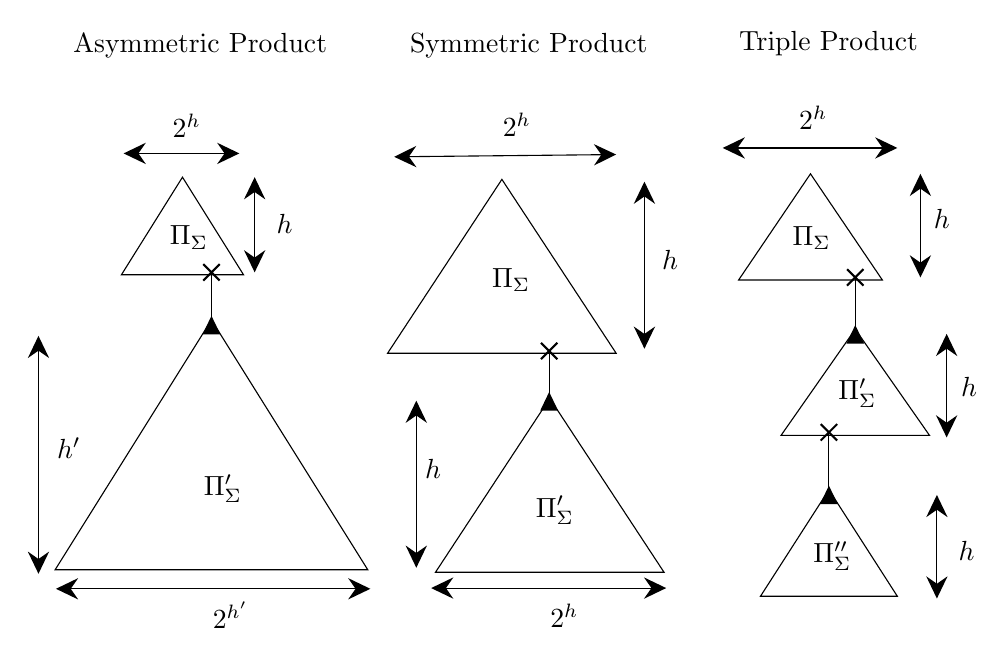
\begin{tikzpicture}[x=0.75pt,y=0.75pt,yscale=-1,xscale=1]
%uncomment if require: \path (0,363); %set diagram left start at 0, and has height of 363

%Flowchart: Extract [id:dp026014598927840638] 
\draw   (78.18,128.94) -- (107.59,175.94) -- (48.78,175.94) -- cycle ;
%Straight Lines [id:da5136161275872781] 
\draw    (52.83,117.48) -- (102.58,117.48) ;
\draw [shift={(105.58,117.48)}, rotate = 180] [fill={rgb, 255:red, 0; green, 0; blue, 0 }  ][line width=0.08]  [draw opacity=0] (10.72,-5.15) -- (0,0) -- (10.72,5.15) -- (7.12,0) -- cycle    ;
\draw [shift={(49.83,117.48)}, rotate = 0] [fill={rgb, 255:red, 0; green, 0; blue, 0 }  ][line width=0.08]  [draw opacity=0] (10.72,-5.15) -- (0,0) -- (10.72,5.15) -- (7.12,0) -- cycle    ;
%Straight Lines [id:da7418298136504138] 
\draw    (112.95,171.79) -- (112.95,131.94) ;
\draw [shift={(112.95,128.94)}, rotate = 450] [fill={rgb, 255:red, 0; green, 0; blue, 0 }  ][line width=0.08]  [draw opacity=0] (10.72,-5.15) -- (0,0) -- (10.72,5.15) -- (7.12,0) -- cycle    ;
\draw [shift={(112.95,174.79)}, rotate = 270] [fill={rgb, 255:red, 0; green, 0; blue, 0 }  ][line width=0.08]  [draw opacity=0] (10.72,-5.15) -- (0,0) -- (10.72,5.15) -- (7.12,0) -- cycle    ;
%Flowchart: Extract [id:dp6454688805946203] 
\draw   (92.15,197.72) -- (167.46,318.08) -- (16.83,318.08) -- cycle ;
%Straight Lines [id:da9054941544395627] 
\draw    (20.22,327.25) -- (165.7,327.25) ;
\draw [shift={(168.7,327.25)}, rotate = 180] [fill={rgb, 255:red, 0; green, 0; blue, 0 }  ][line width=0.08]  [draw opacity=0] (10.72,-5.15) -- (0,0) -- (10.72,5.15) -- (7.12,0) -- cycle    ;
\draw [shift={(17.22,327.25)}, rotate = 0] [fill={rgb, 255:red, 0; green, 0; blue, 0 }  ][line width=0.08]  [draw opacity=0] (10.72,-5.15) -- (0,0) -- (10.72,5.15) -- (7.12,0) -- cycle    ;
%Straight Lines [id:da34661639960721846] 
\draw    (8.8,317.02) -- (8.8,208.39) ;
\draw [shift={(8.8,205.39)}, rotate = 450] [fill={rgb, 255:red, 0; green, 0; blue, 0 }  ][line width=0.08]  [draw opacity=0] (10.72,-5.15) -- (0,0) -- (10.72,5.15) -- (7.12,0) -- cycle    ;
\draw [shift={(8.8,320.02)}, rotate = 270] [fill={rgb, 255:red, 0; green, 0; blue, 0 }  ][line width=0.08]  [draw opacity=0] (10.72,-5.15) -- (0,0) -- (10.72,5.15) -- (7.12,0) -- cycle    ;
%Straight Lines [id:da36867642449433324] 
\draw    (92.15,174.79) -- (92.15,196.72) ;
\draw [shift={(92.15,195.72)}, rotate = 90] [fill={rgb, 255:red, 0; green, 0; blue, 0 }  ][line width=0.08]  [draw opacity=0] (8.93,-4.29) -- (0,0) -- (8.93,4.29) -- cycle    ;
\draw [shift={(92.15,174.79)}, rotate = 135] [color={rgb, 255:red, 0; green, 0; blue, 0 }  ][line width=0.75]    (-5.59,0) -- (5.59,0)(0,5.59) -- (0,-5.59)   ;
%Flowchart: Extract [id:dp23352207486603738] 
\draw   (232.07,130) -- (287.12,213.76) -- (177.01,213.76) -- cycle ;
%Straight Lines [id:da48230532640239776] 
\draw    (183.16,119.09) -- (284.12,118.06) ;
\draw [shift={(287.12,118.03)}, rotate = 539.4200000000001] [fill={rgb, 255:red, 0; green, 0; blue, 0 }  ][line width=0.08]  [draw opacity=0] (10.72,-5.15) -- (0,0) -- (10.72,5.15) -- (7.12,0) -- cycle    ;
\draw [shift={(180.16,119.12)}, rotate = 359.42] [fill={rgb, 255:red, 0; green, 0; blue, 0 }  ][line width=0.08]  [draw opacity=0] (10.72,-5.15) -- (0,0) -- (10.72,5.15) -- (7.12,0) -- cycle    ;
%Straight Lines [id:da3179065072075995] 
\draw    (300.75,208.59) -- (300.75,134.09) ;
\draw [shift={(300.75,131.09)}, rotate = 450] [fill={rgb, 255:red, 0; green, 0; blue, 0 }  ][line width=0.08]  [draw opacity=0] (10.72,-5.15) -- (0,0) -- (10.72,5.15) -- (7.12,0) -- cycle    ;
\draw [shift={(300.75,211.59)}, rotate = 270] [fill={rgb, 255:red, 0; green, 0; blue, 0 }  ][line width=0.08]  [draw opacity=0] (10.72,-5.15) -- (0,0) -- (10.72,5.15) -- (7.12,0) -- cycle    ;
%Straight Lines [id:da3851116063905706] 
\draw    (254.85,212.68) -- (254.85,233.43) ;
\draw [shift={(254.85,232.43)}, rotate = 90] [fill={rgb, 255:red, 0; green, 0; blue, 0 }  ][line width=0.08]  [draw opacity=0] (8.93,-4.29) -- (0,0) -- (8.93,4.29) -- cycle    ;
\draw [shift={(254.85,212.68)}, rotate = 135] [color={rgb, 255:red, 0; green, 0; blue, 0 }  ][line width=0.75]    (-5.59,0) -- (5.59,0)(0,5.59) -- (0,-5.59)   ;
%Flowchart: Extract [id:dp544592078958481] 
\draw   (255.14,235.52) -- (310.19,319.29) -- (200.08,319.29) -- cycle ;
%Straight Lines [id:da2809220248736448] 
\draw    (200.99,326.9) -- (308.24,326.9) ;
\draw [shift={(311.24,326.9)}, rotate = 180] [fill={rgb, 255:red, 0; green, 0; blue, 0 }  ][line width=0.08]  [draw opacity=0] (10.72,-5.15) -- (0,0) -- (10.72,5.15) -- (7.12,0) -- cycle    ;
\draw [shift={(197.99,326.9)}, rotate = 0] [fill={rgb, 255:red, 0; green, 0; blue, 0 }  ][line width=0.08]  [draw opacity=0] (10.72,-5.15) -- (0,0) -- (10.72,5.15) -- (7.12,0) -- cycle    ;
%Straight Lines [id:da7740876724312342] 
\draw    (190.84,314.11) -- (190.84,239.61) ;
\draw [shift={(190.84,236.61)}, rotate = 450] [fill={rgb, 255:red, 0; green, 0; blue, 0 }  ][line width=0.08]  [draw opacity=0] (10.72,-5.15) -- (0,0) -- (10.72,5.15) -- (7.12,0) -- cycle    ;
\draw [shift={(190.84,317.11)}, rotate = 270] [fill={rgb, 255:red, 0; green, 0; blue, 0 }  ][line width=0.08]  [draw opacity=0] (10.72,-5.15) -- (0,0) -- (10.72,5.15) -- (7.12,0) -- cycle    ;
%Flowchart: Extract [id:dp8452267338181432] 
\draw   (380.75,127.32) -- (415.38,178.48) -- (346.12,178.48) -- cycle ;
%Straight Lines [id:da6944629196707921] 
\draw    (341.47,114.85) -- (419.61,114.85) ;
\draw [shift={(422.61,114.85)}, rotate = 180] [fill={rgb, 255:red, 0; green, 0; blue, 0 }  ][line width=0.08]  [draw opacity=0] (10.72,-5.15) -- (0,0) -- (10.72,5.15) -- (7.12,0) -- cycle    ;
\draw [shift={(338.47,114.85)}, rotate = 0] [fill={rgb, 255:red, 0; green, 0; blue, 0 }  ][line width=0.08]  [draw opacity=0] (10.72,-5.15) -- (0,0) -- (10.72,5.15) -- (7.12,0) -- cycle    ;
%Straight Lines [id:da1819515559996132] 
\draw    (433.72,174.23) -- (433.72,130.32) ;
\draw [shift={(433.72,127.32)}, rotate = 450] [fill={rgb, 255:red, 0; green, 0; blue, 0 }  ][line width=0.08]  [draw opacity=0] (10.72,-5.15) -- (0,0) -- (10.72,5.15) -- (7.12,0) -- cycle    ;
\draw [shift={(433.72,177.23)}, rotate = 270] [fill={rgb, 255:red, 0; green, 0; blue, 0 }  ][line width=0.08]  [draw opacity=0] (10.72,-5.15) -- (0,0) -- (10.72,5.15) -- (7.12,0) -- cycle    ;
%Straight Lines [id:da40890931708095946] 
\draw    (402.33,177.23) -- (402.33,201.18) ;
\draw [shift={(402.33,200.18)}, rotate = 90] [fill={rgb, 255:red, 0; green, 0; blue, 0 }  ][line width=0.08]  [draw opacity=0] (8.93,-4.29) -- (0,0) -- (8.93,4.29) -- cycle    ;
\draw [shift={(402.33,177.23)}, rotate = 135] [color={rgb, 255:red, 0; green, 0; blue, 0 }  ][line width=0.75]    (-5.59,0) -- (5.59,0)(0,5.59) -- (0,-5.59)   ;
%Flowchart: Extract [id:dp019118784600717476] 
\draw   (402.33,202.18) -- (438.1,253.34) -- (366.57,253.34) -- cycle ;
%Straight Lines [id:da00657557714538326] 
\draw    (446.36,251.34) -- (446.36,207.43) ;
\draw [shift={(446.36,204.43)}, rotate = 450] [fill={rgb, 255:red, 0; green, 0; blue, 0 }  ][line width=0.08]  [draw opacity=0] (10.72,-5.15) -- (0,0) -- (10.72,5.15) -- (7.12,0) -- cycle    ;
\draw [shift={(446.36,254.34)}, rotate = 270] [fill={rgb, 255:red, 0; green, 0; blue, 0 }  ][line width=0.08]  [draw opacity=0] (10.72,-5.15) -- (0,0) -- (10.72,5.15) -- (7.12,0) -- cycle    ;
%Straight Lines [id:da738808546977765] 
\draw    (389.63,251.86) -- (389.63,278.54) ;
\draw [shift={(389.63,277.54)}, rotate = 90] [fill={rgb, 255:red, 0; green, 0; blue, 0 }  ][line width=0.08]  [draw opacity=0] (8.93,-4.29) -- (0,0) -- (8.93,4.29) -- cycle    ;
\draw [shift={(389.63,251.86)}, rotate = 135] [color={rgb, 255:red, 0; green, 0; blue, 0 }  ][line width=0.75]    (-5.59,0) -- (5.59,0)(0,5.59) -- (0,-5.59)   ;
%Flowchart: Extract [id:dp7765005950494317] 
\draw   (389.63,279.54) -- (422.6,330.85) -- (356.66,330.85) -- cycle ;
%Straight Lines [id:da6620905717679875] 
\draw    (441.66,328.94) -- (441.66,285.03) ;
\draw [shift={(441.66,282.03)}, rotate = 450] [fill={rgb, 255:red, 0; green, 0; blue, 0 }  ][line width=0.08]  [draw opacity=0] (10.72,-5.15) -- (0,0) -- (10.72,5.15) -- (7.12,0) -- cycle    ;
\draw [shift={(441.66,331.94)}, rotate = 270] [fill={rgb, 255:red, 0; green, 0; blue, 0 }  ][line width=0.08]  [draw opacity=0] (10.72,-5.15) -- (0,0) -- (10.72,5.15) -- (7.12,0) -- cycle    ;

% Text Node
\draw (70.81,151.21) node [anchor=north west][inner sep=0.75pt]    {$\Pi _{\Sigma }$};
% Text Node
\draw (72.21,97.22) node [anchor=north west][inner sep=0.75pt]    {$2^{h}$};
% Text Node
\draw (122.25,145.72) node [anchor=north west][inner sep=0.75pt]    {$h$};
% Text Node
\draw (87.17,270.95) node [anchor=north west][inner sep=0.75pt]    {$\Pi _{\Sigma }^{\prime }$};
% Text Node
\draw (91.56,332.45) node [anchor=north west][inner sep=0.75pt]    {$2^{h^{\prime }}$};
% Text Node
\draw (16.46,253.37) node [anchor=north west][inner sep=0.75pt]    {$h^{\prime }$};
% Text Node
\draw (226.09,171.8) node [anchor=north west][inner sep=0.75pt]    {$\Pi _{\Sigma }$};
% Text Node
\draw (231.26,96.89) node [anchor=north west][inner sep=0.75pt]    {$2^{h}$};
% Text Node
\draw (307.95,162.66) node [anchor=north west][inner sep=0.75pt]    {$h$};
% Text Node
\draw (247.21,281.37) node [anchor=north west][inner sep=0.75pt]    {$\Pi _{\Sigma }^{\prime }$};
% Text Node
\draw (254.18,333.31) node [anchor=north west][inner sep=0.75pt]    {$2^{h}$};
% Text Node
\draw (193.86,263.69) node [anchor=north west][inner sep=0.75pt]    {$h$};
% Text Node
\draw (370.83,151.26) node [anchor=north west][inner sep=0.75pt]    {$\Pi _{\Sigma }$};
% Text Node
\draw (374.04,93.38) node [anchor=north west][inner sep=0.75pt]    {$2^{h}$};
% Text Node
\draw (438.94,143.03) node [anchor=north west][inner sep=0.75pt]    {$h$};
% Text Node
\draw (392.97,224.82) node [anchor=north west][inner sep=0.75pt]    {$\Pi _{\Sigma }^{\prime }$};
% Text Node
\draw (452.07,224.14) node [anchor=north west][inner sep=0.75pt]    {$h$};
% Text Node
\draw (380.85,303.49) node [anchor=north west][inner sep=0.75pt]    {$\Pi _{\Sigma }^{\prime \prime }$};
% Text Node
\draw (450.87,303.24) node [anchor=north west][inner sep=0.75pt]    {$h$};
% Text Node
\draw (24.37,58.1) node [anchor=north west][inner sep=0.75pt]   [align=left] {Asymmetric Product};
% Text Node
\draw (186.54,58.1) node [anchor=north west][inner sep=0.75pt]   [align=left] {Symmetric Product};
% Text Node
\draw (345.06,57.17) node [anchor=north west][inner sep=0.75pt]   [align=left] {Triple Product};


\end{tikzpicture}
    \caption{A diagram of the different schemes using variations of products of the sum composition $\Pi_\Sigma$ represented as triangles (suggestive of the Merkle tree structure where the root is at the top and the leaves are at the bottom).  The vertical axis indicates the depth of the trees and the horizontal axis indicates the time steps of each respective sum composition.  In each setup the topmost scheme is the parent that authenticates the child scheme underneath it, e.g. the triple product scheme would be written as $\Pi_\Sigma^\otimes = \Pi_\Sigma \otimes \Pi_\Sigma^\prime \otimes \Pi_\Sigma^{\prime\prime}$.  The lowermost child scheme signs the messages in the overall product composition and the other witness signatures authenticate the time step.}
    \label{Fig:products}
\end{scheme}

%KeyGenProduct
\begin{algorithm}
\caption{$\mathsf{KeyGenProduct}: s,h_1,h_2 \to \mathsf{\hyperref[def:ProductKey]{ProductKey}}  $}\label{alg:KeyGenProduct}
\begin{algorithmic}[1]
\Require $s \in \{0,1\}^\ell$, $h_2\in \mathbb{N}_0$, $h_2\in \mathbb{N}_0$
\State $(s_1,s_2) \gets \mathsf{\hyperref[alg:DoublingPRNG]{DoublingPRNG}}(s)$
\State $(s_3,s_4) \gets \mathsf{\hyperref[alg:DoublingPRNG]{DoublingPRNG}}(s_2)$
\State $\tau_1 \gets \mathsf{\hyperref[alg:KeyGenSum]{KeyGenSum}}(s_1,h_1)$
\State $\tau_2 \gets \mathsf{\hyperref[alg:KeyGenSum]{KeyGenSum}}(s_3,h_2)$
\State $R_2\gets \mathsf{\hyperref[alg:VerificationKeySum]{VerificationKeySum}}(\tau_2)$
\State $\sigma_1 \gets \mathsf{\hyperref[alg:SignSum]{SignSum}}(\tau_1,R_2)$
\State $\tau^\prime_1\gets\mathsf{\hyperref[alg:EraseLeafSK]{EraseLeafSK}}(\tau_1)$
\State \Return $\mathsf{\hyperref[def:ProductKey]{ProductKey}}(\tau_1^\prime,\sigma_1,s_4,\tau_2)$
\end{algorithmic}
\end{algorithm}

%VerificationKeyProduct
\begin{algorithm}
\caption{$\mathsf{VerificationKeyProduct}:\kappa\to \{0,1\}^\ell  $}\label{alg:VerificationKeyProduct}
\begin{algorithmic}[1]
\Require $\kappa \in \mathsf{\hyperref[def:ProductKey]{ProductKey}}$
\State $\mathsf{\hyperref[def:ProductKey]{ProductKey}}[\tau_1,\Sigma,s,\tau_2]\gets \kappa$
\State \Return $\mathsf{\hyperref[alg:VerificationKeySum]{VerificationKeySum}}(\tau_1)$
\end{algorithmic}
\end{algorithm}

%KeyTimeProduct
\begin{algorithm}
\caption{$\mathsf{KeyTimeProduct}: \kappa \to \mathbb{N}_0  $}\label{alg:KeyTimeProduct}
\begin{algorithmic}[1]
\Require $\kappa \in \mathsf{\hyperref[def:ProductKey]{ProductKey}}$
\State $\mathsf{\hyperref[def:ProductKey]{ProductKey}}[\tau_1,\Sigma,s,\tau_2]\gets \kappa$
\State $h_2\gets \mathsf{\hyperref[alg:Height]{Height}}(\tau_2)$
\State $t_1\gets \mathsf{\hyperref[alg:KeyTimeSum]{KeyTimeSum}}(\tau_1)$
\State $t_2\gets \mathsf{\hyperref[alg:KeyTimeSum]{KeyTimeSum}}(\tau_2)$
\State \Return $t_1 2^{h_2}+t_2$
\end{algorithmic}
\end{algorithm}

%SignProduct
\begin{algorithm}
\caption{$\mathsf{SignProduct}: \kappa,m \to \mathsf{\hyperref[def:ProductSignature]{ProductSignature}}  $}\label{alg:SignProduct}
\begin{algorithmic}[1]
\Require $\kappa \in \mathsf{\hyperref[def:ProductKey]{ProductKey}}$, $m\in\{0,1\}^*$
\State $\mathsf{\hyperref[def:ProductKey]{ProductKey}}[\tau_1,\sigma_1,s,\tau_2]\gets \kappa$
\State $\sigma_2\gets \mathsf{\hyperref[alg:SignSum]{SignSum}}(\tau_2,m)$
\State $R_2 \gets \mathsf{\hyperref[alg:VerificationKeySum]{VerificationKeySum}}(\tau_2)$
\State \Return $\mathsf{\hyperref[def:ProductSignature]{ProductSignature}}[\sigma_1,\sigma_2,R_2]$
\end{algorithmic}
\end{algorithm}

%VerifyProduct
\begin{algorithm}
\caption{$\mathsf{VerifyProductSignature}: R,\Sigma,t,m \to \{\mathbf{true},\mathbf{false}\} $}\label{alg:VerifyProductSignature}
\begin{algorithmic}[1]
\Require $R\in\{0,1\}^\ell$, $\Sigma \in \mathsf{\hyperref[def:ProductSignature]{ProductSignature}}$, $t\in \mathbb{N}_0$,  $m\in\{0,1\}^*$
\State $\mathsf{\hyperref[def:ProductSignature]{ProductSignature}}[\sigma_1,\sigma_2,R_2]\gets \Sigma$
\State $\mathsf{\hyperref[def:SumSignature]{SumSignature}}[vk,\sigma,W] \gets \sigma_2$
\State $h_2 \gets \mathrm{length}(W)$
\State $t_1 \gets t / 2^{h_2}$
\State $t_2 \gets t \bmod 2^{h_2}$
\State $b_1 \gets \mathsf{\hyperref[alg:VerifySumSignature]{VerifySumSignature}}(R, \sigma_1, t_1, R_2)$
\State $b_2 \gets \mathsf{\hyperref[alg:VerifySumSignature]{VerifySumSignature}}(R_2, \sigma_2, t_2, m)$
\State \Return $b_1 \wedge b_2$
\end{algorithmic}
\end{algorithm}

%EraseLeafSK
\begin{algorithm}
\caption{$\mathsf{EraseLeafSK}: n \to \mathsf{\hyperref[def:Node]{Node}}  $}\label{alg:EraseLeafSK}
\begin{algorithmic}[1]
\Require $n\in \mathcal{T}$
\State $\mathsf{\hyperref[def:Node]{Node}}[v,l,r] \gets n$
\If{$\mathsf{\hyperref[alg:IsLeaf]{IsLeaf}}(n)$}
    \State $(sk,vk)\gets v$
    \State \Return $\mathsf{\hyperref[def:Node]{Node}}[(\mathrm{null}, vk ), \mathrm{null}, \mathrm{null}]$
\Else
    \If{$ l = \mathrm{null} \wedge r\in\mathcal{T}$}
        \State \Return $\mathsf{\hyperref[def:Node]{Node}}[v,\mathrm{null},\mathsf{\hyperref[alg:EraseLeafSK]{EraseLeafSK}}(r)]$
    \Else
        \State \Return $\mathsf{\hyperref[def:Node]{Node}}[v,\mathsf{\hyperref[alg:EraseLeafSK]{EraseLeafSK}}(l),\mathrm{null}]$
    \EndIf
\EndIf
\end{algorithmic}
\end{algorithm}


%KeyUpdateProduct
\begin{algorithm}
\caption{$\mathsf{KeyUpdateProduct}:\kappa , t \to \mathsf{\hyperref[def:ProductKey]{ProductKey}}  $}\label{alg:KeyUpdateProduct}
\begin{algorithmic}[1]
\Require $\kappa \in \mathsf{\hyperref[def:ProductKey]{ProductKey}}$, $t\in \mathbb{N}_0$
\State $\mathsf{\hyperref[def:ProductKey]{ProductKey}}[\tau_1,\sigma_1,s,\tau_2]\gets \kappa$
\State $t_\mathrm{key} \gets \mathsf{\hyperref[alg:KeyTimeProduct]{KeyTimeProduct}}(\kappa)$
\State $h_1\gets \mathsf{\hyperref[alg:Height]{Height}}(\tau_1)$
\State $h_2\gets \mathsf{\hyperref[alg:Height]{Height}}(\tau_2)$
\If{$t>t_\mathrm{key} \wedge t<2^{h_1+h_2}$}
    \State $i \gets \mathsf{\hyperref[alg:KeyTimeSum]{KeyTimeSum}}(\tau_1)$
    \State $t_1 \gets t / 2^{h_2}$
    \State $t_2 \gets t \bmod 2^{h_2}$
    \If{$i < t_1$}
        \State $s_1 \gets \mathrm{null}$
        \State $s_2 \gets s$
        \While {$i < t_1$}
            \State $(s_1,s_2) \gets \mathsf{\hyperref[alg:DoublingPRNG]{DoublingPRNG}}(s_2)$
            \State $i \gets i + 1 $
        \EndWhile
        \State $\tau^\prime_1\gets\mathsf{\hyperref[alg:EvolveKey]{EvolveKey}}(\tau_1,t_1)$
        \State $\tau^\prime_2 \gets \mathsf{\hyperref[alg:KeyGenSum]{KeyGenSum}}(s_1,h_2)$
        \State $R_2^\prime\gets \mathsf{\hyperref[alg:VerificationKeySum]{VerificationKeySum}}(\tau^\prime_2)$
        \State $\sigma_1^\prime \gets \mathsf{\hyperref[alg:SignSum]{SignSum}}(\tau^\prime_1,R_2^\prime)$
        \State $\tau^\prime_2\gets\mathsf{\hyperref[alg:EvolveKey]{EvolveKey}}(\tau^\prime_2,t_2)$
        \State $\tau_1^{\prime\prime} \gets \mathsf{\hyperref[alg:EraseLeafSK]{EraseLeafSK}}(\tau^\prime_1,t_1)$
        \State \Return $\mathsf{\hyperref[def:ProductKey]{ProductKey}}[\tau^{\prime\prime}_1,\sigma_1^\prime,s_2,\tau^\prime_2]$
    \Else
        \State $\tau^\prime_2\gets\mathsf{\hyperref[alg:KeyUpdateSum]{KeyUpdateSum}}(\tau_2,t_2)$
        \State \Return $\mathsf{\hyperref[def:ProductKey]{ProductKey}}[\tau_1,\sigma_1,s,\tau^\prime_2]$
    \EndIf
\Else
    \State \Return $\kappa$
\EndIf
\end{algorithmic}
\end{algorithm}


\newpage
\section{Linear KES Scheme}

This section specifies the linear scheme in a key-evolving setup.  
Figure~\ref{Fig:Lscheme} shows a schematic of the key cache and set of verification keys.
The indexing scheme may be designed in a way that provides practically any number of time steps, but to maintain forward security secret keys have to be erased after they are used to make signatures. 

%Key Sets
\begin{scheme}
\centering
\tikzset{every picture/.style={line width=0.75pt}} %set default line width to 0.75pt    
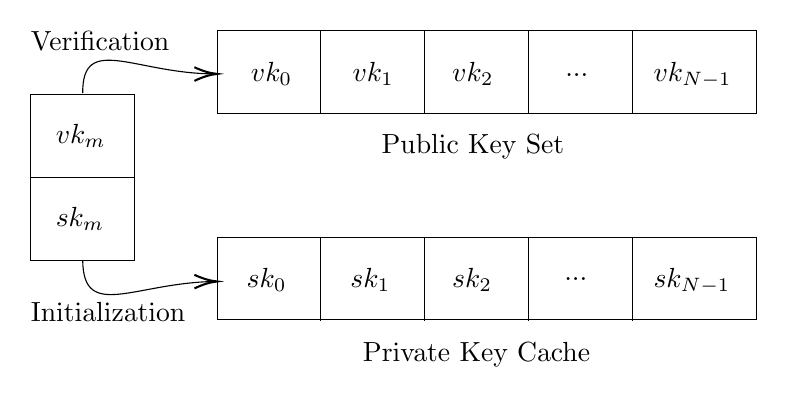
\begin{tikzpicture}[x=0.75pt,y=0.75pt,yscale=-1,xscale=1]
%uncomment if require: \path (0,904); %set diagram left start at 0, and has height of 904

%Shape: Rectangle [id:dp682369958224049] 
\draw   (130,439) -- (390,439) -- (390,479) -- (130,479) -- cycle ;
%Shape: Rectangle [id:dp029105315478833438] 
\draw   (130,539) -- (390,539) -- (390,578.25) -- (130,578.25) -- cycle ;
%Straight Lines [id:da8664832655580454] 
\draw    (180,539) -- (180,579) ;
%Straight Lines [id:da21940897523365077] 
\draw    (230,539) -- (230,579) ;
%Straight Lines [id:da061577667585936746] 
\draw    (280,539) -- (280,579) ;
%Straight Lines [id:da9606028506580655] 
\draw    (330,539) -- (330,579) ;
%Straight Lines [id:da33309348645795556] 
\draw    (180,439) -- (180,479) ;
%Straight Lines [id:da09310707053010914] 
\draw    (230,439) -- (230,479) ;
%Straight Lines [id:da4978709509088688] 
\draw    (280,439) -- (280,479) ;
%Straight Lines [id:da49759389076599403] 
\draw    (330,439) -- (330,479) ;
%Shape: Rectangle [id:dp04310477297760196] 
\draw   (40,470) -- (90,470) -- (90,550) -- (40,550) -- cycle ;
%Straight Lines [id:da5179804493397875] 
\draw    (40,510) -- (90,510) ;
%Curve Lines [id:da44792008270465455] 
\draw    (65.25,469.25) .. controls (65,440.44) and (89.98,459.65) .. (128.24,460) ;
\draw [shift={(130,460)}, rotate = 539.64] [color={rgb, 255:red, 0; green, 0; blue, 0 }  ][line width=0.75]    (10.93,-3.29) .. controls (6.95,-1.4) and (3.31,-0.3) .. (0,0) .. controls (3.31,0.3) and (6.95,1.4) .. (10.93,3.29)   ;
%Curve Lines [id:da656674428921332] 
\draw    (65.25,550) .. controls (65.66,578.89) and (90,560.81) .. (128.24,560.02) ;
\draw [shift={(130,560)}, rotate = 539.64] [color={rgb, 255:red, 0; green, 0; blue, 0 }  ][line width=0.75]    (10.93,-3.29) .. controls (6.95,-1.4) and (3.31,-0.3) .. (0,0) .. controls (3.31,0.3) and (6.95,1.4) .. (10.93,3.29)   ;


% Text Node
\draw (39,438) node [anchor=north west][inner sep=0.75pt]   [align=left] {Verification};
% Text Node
\draw (39,569) node [anchor=north west][inner sep=0.75pt]   [align=left] {Initialization};
% Text Node
\draw (208,488) node [anchor=north west][inner sep=0.75pt]   [align=left] {Public Key Set};
% Text Node
\draw (51,523) node [anchor=north west][inner sep=0.75pt]    {$sk_{m}$};
% Text Node
\draw (51,483) node [anchor=north west][inner sep=0.75pt]    {$vk_{m}$};
% Text Node
\draw (199,588) node [anchor=north west][inner sep=0.75pt]   [align=left] {Private Key Cache};
% Text Node
\draw (145,453) node [anchor=north west][inner sep=0.75pt]    {$vk_{0}$};
% Text Node
\draw (296.5,458.5) node [anchor=north west][inner sep=0.75pt]    {$...$};
% Text Node
\draw (339,453) node [anchor=north west][inner sep=0.75pt]    {$vk_{N-1}$};
% Text Node
\draw (242,453) node [anchor=north west][inner sep=0.75pt]    {$vk_{2}$};
% Text Node
\draw (194,453) node [anchor=north west][inner sep=0.75pt]    {$vk_{1}$};
% Text Node
\draw (296,557) node [anchor=north west][inner sep=0.75pt]    {$...$};
% Text Node
\draw (339,552.25) node [anchor=north west][inner sep=0.75pt]    {$sk_{N-1}$};
% Text Node
\draw (242,552.25) node [anchor=north west][inner sep=0.75pt]    {$sk_{2}$};
% Text Node
\draw (193,552.25) node [anchor=north west][inner sep=0.75pt]    {$sk_{1}$};
% Text Node
\draw (143,552.25) node [anchor=north west][inner sep=0.75pt]    {$sk_{0}$};


\end{tikzpicture}

    \caption{A diagram showing the key sets in a setup where there are $N$ total time steps.  Upon initialization, a key pair $sk_m$ and $vk_m$ is chosen at random.  $sk_m$ is used to sign the key cache during initialization and then $sk_m$ is securely erased.  Signatures are produced from the private key cache $\{sk_{m/i}:0\leq i<N\}$ and each time step corresponds to an index $i$.  As time increments, secure erasure in time step $t$ corresponds to setting the private key cache to $\{sk_{m/i}:t\leq i<N\}$ and erasing $\{sk_{m/i}:0\leq i<t\}$.  The public key is included in signatures and authenticated with a signature produced by $sk_m$ that verifies with $vk_m$. }
    \label{Fig:Lscheme}
\end{scheme}

\begin{scheme}
\begin{adjustbox}{minipage=\linewidth,fbox,center}
{\centering{\bf Linear KES Protocol $\Pi_{\mathrm{L}}$:} \par} { \raggedright
    The protocol is run by a registered set of parties $\mathcal{P}$ denoted by $U_i\in\mathcal{P}$ interacting with a singer $U_S$ as follows:
    
    \noindent\rule{\textwidth}{.5pt}
    \noindent  \textbf{Key Generation.}  Upon receiving the message $(\mathsf{KeyGen},sid,U_S,T)$ from $U_S$ if $T>0$, $U_S$ does the following, otherwise ignore the input:  
    pick a random $s_m\in \{0,1\}^{\ell}$ then compute $(sk_m,vk_m) \gets \mathsf{\hyperref[def:KeyGen]{KeyGen}}(s_m)$. 
    For each $i\in \{j: 0 \leq j < T\}$ pick a random $s_i$ and compute $(sk_i,vk_i) \gets \mathsf{\hyperref[def:KeyGen]{KeyGen}}(s_i)$ then add $(sk_i,vk_i)$ to set $\mathbb{K}$ and securely erase $s_i$.
    For each key pair $(sk_i,vk_i)\in \mathbb{K}$ compute $\sigma_i \gets \mathsf{\hyperref[def:Sign]{Sign}}(sk_m,vk_i||i)$,
    then add the tuple $(i,\sigma_i,sk_i,vk_i)$ to the set $\mathbb{S}_m$.
    Record $\mathbb{S}_m$, securely erase $sk_m$, $s_m$ and $\mathbb{K}$. Send the message $(\mathsf{VerificationKey},sid,vk_m)$ to $U_S$.
    
    \noindent\rule{\textwidth}{.5pt}
    \noindent  \textbf{Key Update.}
    Upon receiving the message $(\mathsf{KeyUpdate},sid,U_S,t)$ from $U_S$ with a $sid$ for which it has the signing key set $\mathbb{S}_m$, $U_S$ does the following, otherwise ignore the input: 
    $\forall(i,\sigma_i,sk_i,vk_i)\in\mathbb{S}_m$ such that $i\geq t$, add $(i,\sigma_i,sk_i,vk_i)$ to the set $\mathbb{S}_m^\prime$. 
    Record $\mathbb{S}_m^\prime$ and securely erase $\mathbb{S}_m$. Send the message $(\mathsf{Updated},sid)$ to $U_S$.

    \noindent\rule{\textwidth}{.5pt}
    \noindent \textbf{Signature Creation.}
    Upon receiving the message  $(\mathsf{Sign},sid,U_S,m,t)$ from $U_S$ with a $sid$ for which it has the signing key set $\mathbb{S}_m$ and if $i\geq t$  $\forall(i,\sigma_i,sk_i,vk_i)\in\mathbb{S}_m$ and $\exists (i,\sigma_i,sk_i,vk_i)\in\mathbb{S}_m$ such that $i=t$, $U_S$ does the following, otherwise ignore the input: find the entry $(t,\sigma_{t},sk_t,vk_t)\in\mathbb{S}_m$ and compute $\Sigma_t \gets (\sigma_t,vk_t,\mathsf{\hyperref[def:Sign]{Sign}}(sk_t,m))$, then send the message $(\mathsf{Signature},sid,m,t,\Sigma_t)$ to $U_S$. 
      
    \noindent\rule{\textwidth}{.5pt}
    \noindent  \textbf{Signature Verification.}
    When party $U_i$ receives the message $(\mathsf{Verify},sid,m,t,\Sigma_t,vk_m)$, $U_i$ performs the following: \newline
    Parse the signature as $(\sigma_t,vk_t,\sigma_m) \gets \Sigma_t$ and compute $b\gets \mathsf{\hyperref[def:Verify]{Verify}}(vk_m,\sigma_t,vk_t) \wedge \mathsf{\hyperref[def:Verify]{Verify}}(vk_t,\sigma_m,m)$.   
    $U_i$ outputs the message $(\mathsf{Verified},sid,m,t,b)$.

}
\end{adjustbox}
\caption{The linear KES scheme as a protocol assuming the underlying signing routine in Figure~\ref{Fig:Sign}.}
\label{Fig:protocolLKES}
\end{scheme}


 \section{Test Vectors}
 {\footnotesize
 \begin{verbatim}
----------------------------------------------------------------
Sum Test vectors 1:
seed:
928b20366943e2afd11ebc0eae2e53a93bf177a4fcf35bcc64d503704e65e202
h = 7
sum_key VK:
23d72240b54a6135ec7ca96013d2e4edacefc2ccad2aac861430eeb9286b4ae6
sum_key SK
3fcd949fc91c761887d8bcad1c8b1b1565d25d4ffdbfffa28cb66a51982166a7
4fef963016cf2e19cfa3920ab5bf2a1413f40d527327aeb2d2f0a8298c345b93
9f2ed5b9d1df27926d225f8eb41c426254d4218e054f5c4a102eeccb58876596
0081462dd35671f7b03059a45a216c87bf9d6f66560400a4507ffb8c1cc24b5d
e608f233c14f3362a560aa0c2552c83e054f07c4e849adf8cc39e598c94f6b5e
738592a55902f5f3ab6d2247585c5472c1d9f2132481a3d5cc39a7ff5edf4354
9100f3bfcc733fd6321b36a47efec3adfc6a98980e7c4b817656f5ad9a1f04e8
1c55e1e61aa043c4ea026bcfb8e135af41037bd966f0591b0644fa969cdb8c48
df3f8be89df4800275fcaf3426ce8f3b0318cc19a23274474e74e56c6d38d6ad
03a00051ca63483351a1439d2971881aaf11c3bd27223e819ab1a2b42775bd30
99c56c8b88e3730f40d7aca97cbc7ae8c5da87fe004445e711233b0a8d2f1952
b79655490975d0f3d5a6a99e1302a2adbff0604441f13c6b13f6d99e45d51532
ba0dae00769f36ce8cf5c3d2d9ae8d9a0f3b459ddff8cb49409c7a509ad1b40f
f67b7fd237f198218bba90c6bee38c54d657f407097ddc2f2afb04da23187f91
5e9f68cf1c62dc579ea9b9aae5ca65998256f5a702c9cea2125f24927efd92ee
97777705002de49bc5e38e8afbeffa60043bf5f45107608537bf8a8fd93f08f4
eb2dffb06ccf6830ae3daac66a03ae7516ddecf1663897d4a3859d89a7d03758
53afbed9a964142027adac58b88711a61e4ca6675d16a02755fb87871d8b676e
cbe829fc8a0013f33ec006608e72d7d951ab9384bf0c5a455dacc0ab206337b5
e92e5b5484ea955ce11603b1ed207b11904e7bec4b5ca1985a64e2e18fd3d109
854403f7bec092897adc1a78d0225cd2a3ec84b94b84ac2cf175b9809aeeebea
18f9958552f0000ac49a2c2f8503d9ba7c2af8d4527acb1fbeaf77d87d151256
d68f202019fb73fce14b4bb0ccc19079263a8115a13fb9cf015c76f16abccb9b
5ce91a9e866e6d
message:
6d657373616765
sigma t = 0:
fce14b4bb0ccc19079263a8115a13fb9cf015c76f16abccb9b5ce91a9e866e6d
90107bbc5a7d6fd9747f6076e107ce2243d635bfa5439af24643465174054201
16c5135c5fa10c9468086fe8d2998a3a04e39efe5971868e4f95fe127ac81709
92897adc1a78d0225cd2a3ec84b94b84ac2cf175b9809aeeebea18f9958552f0
64142027adac58b88711a61e4ca6675d16a02755fb87871d8b676ecbe829fc8a
1c62dc579ea9b9aae5ca65998256f5a702c9cea2125f24927efd92ee97777705
490975d0f3d5a6a99e1302a2adbff0604441f13c6b13f6d99e45d51532ba0dae
8be89df4800275fcaf3426ce8f3b0318cc19a23274474e74e56c6d38d6ad03a0
8592a55902f5f3ab6d2247585c5472c1d9f2132481a3d5cc39a7ff5edf435491
9f2ed5b9d1df27926d225f8eb41c426254d4218e054f5c4a102eeccb58876596
----------------------------------------------------------------
sigma t = 1:
8ad3faaeac74cd22846f2eaefa87d41f520a804c1a8c92d7eca338634e652fbd
d634d8527d79f7ee79ee1f1dfba3aa4da524b45679227ff948304820bc608409
adc1444d9f369b3c1afbb720d27a32397212273f77e7f427570d4ce8a935fe0e
955ce11603b1ed207b11904e7bec4b5ca1985a64e2e18fd3d109854403f7bec0
64142027adac58b88711a61e4ca6675d16a02755fb87871d8b676ecbe829fc8a
1c62dc579ea9b9aae5ca65998256f5a702c9cea2125f24927efd92ee97777705
490975d0f3d5a6a99e1302a2adbff0604441f13c6b13f6d99e45d51532ba0dae
8be89df4800275fcaf3426ce8f3b0318cc19a23274474e74e56c6d38d6ad03a0
8592a55902f5f3ab6d2247585c5472c1d9f2132481a3d5cc39a7ff5edf435491
9f2ed5b9d1df27926d225f8eb41c426254d4218e054f5c4a102eeccb58876596
----------------------------------------------------------------
sigma t = 10:
734b26feb6c78e663e0476985aa6163610f24bfad413aac1dd528fdd810bcf94
682ac31eae1ad22025870097a8ed50d52a81842c53c89a96cc32bcdd5e5df7da
a59154d66209b9d7f1a15c54b4bfd8c852075733b811d75c2a5fe6242e844d02
99280da00680942b45c7ce1face17413e280011bacadf1970099df137f7e23cd
9ee0b4b3911ea215d5936e98cf4b8bc127f9ae304ea078f937d386185e3827dc
f8021233d3de0d5fc40ac9064e6934a4dafd2a0a442619f7ef02e0e5bac22b8b
8b88e3730f40d7aca97cbc7ae8c5da87fe004445e711233b0a8d2f1952b79655
8be89df4800275fcaf3426ce8f3b0318cc19a23274474e74e56c6d38d6ad03a0
8592a55902f5f3ab6d2247585c5472c1d9f2132481a3d5cc39a7ff5edf435491
9f2ed5b9d1df27926d225f8eb41c426254d4218e054f5c4a102eeccb58876596
----------------------------------------------------------------
sigma t = 100:
31439986a2c4a60f2c21b8ef73714305b97212ed69c539d804310df2dd2fa937
66de8606af1ad8d39eaf0374ed195df9d883badf968fd5a26295a6e4f390658c
390d3ec1da812a93ad9118a373bf544941073643364f451de0018bd18619cb09
8323964e90a191163d041a65b7892b0ecc0e0f3eb6c0354fc5c24a05567d21b1
4e9903919fa12296699360b7edf2fce299553e29265ac3c63896ca70940b4e1c
eaccd7fd90deae8a2f9998a653acae63a446b372a603ce6bae5a4beaa2df2563
01483655546cbb36fa2dafca28168b3c48969664e4c1d4ee90306a2e111f4ce3
67a86e2d941dc917affb31ffe23bf21fb7e5716bda7b351bd69277212be33d0e
6f75812121ddf093a6195d93bb6aca4a9e0340cdb4188857f8681b758be28a52
4fef963016cf2e19cfa3920ab5bf2a1413f40d527327aeb2d2f0a8298c345b93
----------------------------------------------------------------
Sum Test vectors 2:
seed:
45f3d3ed97ca49b86f1ae514e55e69e0fba32124aa23eb4b70260f89f259271b
h = 2
sum_key VK:
f7048e1396222415e93193e78bed2c309c29e11996989a467dda416030be6271
sum_key SK
3fcd949fc91c761887d8bcad1c8b1b1565d25d4ffdbfffa28cb66a51982166a7
abb00c9449578442a966f6e2482a454608f2536d90cd912db7a67bec7fd8c5a4
e6c4fad6f115d1c24da11a42fe1e9ad893ecede63d661e8cf4207b182cbcc124
0081462dd35671f7b03059a45a216c87bf9d6f66560400a4507ffb8c1cc24b5d
e6a67aa79f856ce1268d48fdf659354ccc70c383eca31afec8978c82c770b0eb
d9306ab72a51abb7736951b9bb8760ee608219f456c99b765a4f2ff46a59895c
3c0043bf34984ca18ab206ef31241a0b95aa74b1a70cf3749999a4906e601a86
cf8950cd517ae5d9118bef024e4947feca04c893636370ca973958b8e8fc784b
add4
message:
6d657373616765
----------------------------------------------------------------
sigma t = 0:
50cd517ae5d9118bef024e4947feca04c893636370ca973958b8e8fc784badd4
5c4c7bc45754be614a1aaf28c1e271e8c5a3b4378a8fe2fed05bbc7c9f7209d6
deeced944680bb36fe547496592b0a45be3c40ab513bc2ba432ca1e8ed9fa908
306ab72a51abb7736951b9bb8760ee608219f456c99b765a4f2ff46a59895c3c
e6c4fad6f115d1c24da11a42fe1e9ad893ecede63d661e8cf4207b182cbcc124
----------------------------------------------------------------
sigma t = 1:
23805967370c5e2365e6fd6a4ebbf6a815caaabeee9bd1e1f073b168b8604412
b1a594b4d090fcae271587f43c787a7a99ba23bf19c8abc1cb52a614eaa91d99
c6a18eb12eee582358d6f301d81f1e040a2214d19a61d632d7ef38402707b607
a67aa79f856ce1268d48fdf659354ccc70c383eca31afec8978c82c770b0ebd9
e6c4fad6f115d1c24da11a42fe1e9ad893ecede63d661e8cf4207b182cbcc124
----------------------------------------------------------------
sigma t = 2:
f79c37329c6af0fcab56470dd88622780212f1542959d5470e25dcf20c83fb70
b8e9d085839ca0948c7e66fd009efa2c3918f850fb937549a162ef9e140278c0
18ae8147981d6cb7bb35756992fb7afd90473ad292738a7c6e97a93715b1120a
8b4e4e018c976d01d661e0449cf2b351903f4df950d5c26608d527d12fceecae
abb00c9449578442a966f6e2482a454608f2536d90cd912db7a67bec7fd8c5a4
----------------------------------------------------------------
sigma t = 3:
05a5b1306d00c18df680c7fc0791cd0b1f30b96b365bdb2d766a3f621f209d7a
0cad034776232efb95b4732665d2a0477fa107c089b4248fe96c68a3950bbc36
195bb53e13bd7da4ac7f3fd11cad79737901347f88490cb104ddfbb7a695b405
9a94aaf251089e0c6e9d80b5038a2fa24a1fb5d44b82a244fc2416c63c6a93e8
abb00c9449578442a966f6e2482a454608f2536d90cd912db7a67bec7fd8c5a4
----------------------------------------------------------------
Product Test vectors 1:
seed:
928b20366943e2afd11ebc0eae2e53a93bf177a4fcf35bcc64d503704e65e202
h1 = 5
h2 = 9
prod_key VK:
2778dce7717affe951bb5eef6e06bdc2efad4ad12de0a26fefb4dcd17eeb8879
prod_key SK:
0000022581462dd35671f7b03059a45a216c87bf9d6f66560400a4507ffb8c1c
c24b5de602ae690e28498bcc82f35abfffd9df1eeceeddacee9e804c2adf15cf
5846873ff78af2eeea581c8d9528b73c1ad4f1b64c012f6374a14a79f830f52d
3ef478fa00f3bfcc733fd6321b36a47efec3adfc6a98980e7c4b817656f5ad9a
1f04e81c5504d4b53fba001b47f40acb33d7a34b5e52c3d60652fca791747052
e786303399c48c1b5929507328ba3c06778cf01340e5c0f0baa4266011ee7bfa
77f9b8908d0051ca63483351a1439d2971881aaf11c3bd27223e819ab1a2b427
75bd3099c56c58a54679e391ea99f402ce503c2702ce2948db7e7c2d0e2f1216
f85a8df48a8882be9fed061437dbc8e4def34e6b62b0b31b10ad0c12e3a29c6c
127e174b29f900769f36ce8cf5c3d2d9ae8d9a0f3b459ddff8cb49409c7a509a
d1b40ff67b7fd2d430ffcc7e117254c80735690b5e6b0be01d5979ddd5d58ec9
7b67ab4b625f681b09af6bfa67bc552dfe988b195cfc56842b8d2dfd4393cb39
d65ae3f536f444002de49bc5e38e8afbeffa60043bf5f45107608537bf8a8fd9
3f08f4eb2dffb06c2d01c07011e40a2a4c704465a31cf00362fec8f0101d2c0a
90695fe6141e3b9e20c389fdd2a1158838c6a9360613af63b652bbb32e5ddfac
b9d9d3b264bfbad7008d7a246193a6c0b1150ca52eb63056561a8fb9fc2e9a55
707e0ddbe5413b5f835341a0d00b700317420b12614dc34df074b6600c724a0d
6d14e48d5d6b13f1ec000001005341a0d00b700317420b12614dc34df074b660
0c724a0d6d14e48d5d6b13f1ec71df89cc7a3d2efef4dbbea78e218fb02e9822
4e4cf3f3dea03ac33e2126715dc118b182339b6610f0b42422f84fe106bf1547
dc008f536d8e6605a7df659d0f20c389fdd2a1158838c6a9360613af63b652bb
b32e5ddfacb9d9d3b264bfbad71b09af6bfa67bc552dfe988b195cfc56842b8d
2dfd4393cb39d65ae3f536f44482be9fed061437dbc8e4def34e6b62b0b31b10
ad0c12e3a29c6c127e174b29f9c48c1b5929507328ba3c06778cf01340e5c0f0
baa4266011ee7bfa77f9b8908df78af2eeea581c8d9528b73c1ad4f1b64c012f
6374a14a79f830f52d3ef478fa73fb7484a9495b2e7250bf5f240ddaa27e9400
931638c82dd9997164813acedd504dc7313e27d940b927c90d1f2a4f924c86dc
027a0d82254681c8c569cc438a859360f41b1f337e945304fb8f353462312266
051f95bbbf3de5fe85bda0a41c807e42158dae0527d19c29e0de8b674a150600
3b2a0fd56357a3f5262a2c2863005b323037fe19731579cf837081f796fafca0
bf00e088e9ac0f669f00710f1d9e883afce510c55e536fb44e82e24bc8267e72
74fbfc8560c06449e737ffd4c11be073875d9285867946bcc0646682d5714c18
af5d624c34cc1dca780f75f009f700133ab3f97ee7b20c0752360a1a051e5417
46b64381269eee6ca8c6d714f40c774aafbaf11433164d788f5eab6c1ed04536
49a66b0514f69595bd3ad1bc06b8a037dacd2bcff52fe4ab19171fe654d00bad
32b3acefbc3eea81c169111a1bcb0e00b82243777045e2972b31ad050c3b8c20
1c4478e575ef648c3b8146a3c160e539dc0c831fb6e833d3e4aab27360772691
2fb53bd166878b0f077db6f5eb046fe28b2582f4f8859a40c3ed83062341e036
10386b29ffc2c78f19f2e3f1526fec980012f0ab2a290a1e5e6c24c41a3af0a1
31a82dbad6481d26b3be38048ebab471b3c37bb9251f5564c3f290b11bc0bd4d
2c4d78b823281f969715e3ff79505ec9a96c4d456ea6b7d680d8e417d0fac5a8
619096c8cf9d2655e3de0197a598bf6c0400551b316e4d8cacd6165792a8e7b3
df31f273ef6a00fb03c5a3ca17ec045761524350bf6f5936e2eb8ccdb8ebeb46
3ac6f809901eb880fcf72f9342e225d9d3e2d1a8f6080547e22f8c9149245775
7c23070c3e5484ccb926e3c9f9323c13627700cdf3b7485a663dd2c80dd7a22b
2ce9da07ffc6503f4983f51725c1c47b14dc3bff9acae648d41686235891e55a
9bbece0b64caf5ac12a7b1843bcb368e376a529f2f7e4f1bb778edd2cdc618f0
7929a4e837c8f7409f679e56ddf11ce0ea43de008ecfcba1e11dfc8422e10108
8ad2ab04e022049ab3dd98d92ac8643e102b94f27b1feba5c5cfda3c04c12724
07d2b0ee5f59600d72c6d5c058720252a1519d24152b26d8fc94280cb283247c
75eb8a84aeb73bae07cbf93aa0b838cc798fa59e00ff386a80b810e8009d779e
bda6719f94b15f401368dccd6bb9c1040ed6cb7e5d7ca602978e08d06b891a49
2ac6383fe0eeac159245d4ee3be4a83660d554d2ef142f528ba5137889730d25
a2220ce5cfa47b43fa5ff8a63f1de29bd04db0da0300419b5aac9de889955e26
59e5044e8deacc387a966eb2efc3ff7ab37c6ae7f5a23635de621250f44cebe8
bcc3bead7dea8c6dcbb686e38c52ddcb32744000c694
message:
6d657373616765
----------------------------------------------------------------
sigma t = 0:
5341a0d00b700317420b12614dc34df074b6600c724a0d6d14e48d5d6b13f1ec
71df89cc7a3d2efef4dbbea78e218fb02e98224e4cf3f3dea03ac33e2126715d
c118b182339b6610f0b42422f84fe106bf1547dc008f536d8e6605a7df659d0f
20c389fdd2a1158838c6a9360613af63b652bbb32e5ddfacb9d9d3b264bfbad7
1b09af6bfa67bc552dfe988b195cfc56842b8d2dfd4393cb39d65ae3f536f444
82be9fed061437dbc8e4def34e6b62b0b31b10ad0c12e3a29c6c127e174b29f9
c48c1b5929507328ba3c06778cf01340e5c0f0baa4266011ee7bfa77f9b8908d
f78af2eeea581c8d9528b73c1ad4f1b64c012f6374a14a79f830f52d3ef478fa
3635de621250f44cebe8bcc3bead7dea8c6dcbb686e38c52ddcb32744000c694
77afaf41afd853c313ccae12dfe2c0cd748f4f6d934c4326a29fc5ec52289fb6
edda33c37b27a2a124d190f5b8a313b55a4a690a625f8cd2432e14e4b23ba504
142f528ba5137889730d25a2220ce5cfa47b43fa5ff8a63f1de29bd04db0da03
152b26d8fc94280cb283247c75eb8a84aeb73bae07cbf93aa0b838cc798fa59e
9f2f7e4f1bb778edd2cdc618f07929a4e837c8f7409f679e56ddf11ce0ea43de
d1a8f6080547e22f8c91492457757c23070c3e5484ccb926e3c9f9323c136277
6c4d456ea6b7d680d8e417d0fac5a8619096c8cf9d2655e3de0197a598bf6c04
8b2582f4f8859a40c3ed83062341e03610386b29ffc2c78f19f2e3f1526fec98
37dacd2bcff52fe4ab19171fe654d00bad32b3acefbc3eea81c169111a1bcb0e
e073875d9285867946bcc0646682d5714c18af5d624c34cc1dca780f75f009f7
807e42158dae0527d19c29e0de8b674a1506003b2a0fd56357a3f5262a2c2863
7c90e4b7fee6254fd3b19a93da32fe4b38f16b5f16c6362cf5e45d184275bc19
----------------------------------------------------------------
sigma t = 100:
5341a0d00b700317420b12614dc34df074b6600c724a0d6d14e48d5d6b13f1ec
71df89cc7a3d2efef4dbbea78e218fb02e98224e4cf3f3dea03ac33e2126715d
c118b182339b6610f0b42422f84fe106bf1547dc008f536d8e6605a7df659d0f
20c389fdd2a1158838c6a9360613af63b652bbb32e5ddfacb9d9d3b264bfbad7
1b09af6bfa67bc552dfe988b195cfc56842b8d2dfd4393cb39d65ae3f536f444
82be9fed061437dbc8e4def34e6b62b0b31b10ad0c12e3a29c6c127e174b29f9
c48c1b5929507328ba3c06778cf01340e5c0f0baa4266011ee7bfa77f9b8908d
f78af2eeea581c8d9528b73c1ad4f1b64c012f6374a14a79f830f52d3ef478fa
5231ade3d2740ff4bdc287e99a58bd56ec92374864b1d127f1285e157943b0b5
c1a9cc3d4cb081b80be98fbd156085071831d017c2767b0da524c02be80e948a
2fc1365422c55777a9558948d9d14652e3a1371fb10304563f558afd2e228305
e98b22232fc5437eff92b806497809db2f3135ab71b97bc2f805b15235f5f0ca
0daf104308b01c79a7808f543acf0df6567db3d025e45d0d6a0e6055c6e81422
3a9fe793cd40a147ea48be2e9bc1e36ea6e70e9a73c89b84b7188953c381be9b
dca51174175f69fc08b299c66a623c43f7e25eaf987045e633495457dae642a7
27e15fa89c1228ffd59d3a25c533cfd5be827b04b4aae0fbd32f488f8df17fa5
1fee2ef73c4046a6f823eb67a7c7b1172244fb1ecef4ee092bd1232d133dc771
4aafbaf11433164d788f5eab6c1ed0453649a66b0514f69595bd3ad1bc06b8a0
e073875d9285867946bcc0646682d5714c18af5d624c34cc1dca780f75f009f7
807e42158dae0527d19c29e0de8b674a1506003b2a0fd56357a3f5262a2c2863
7c90e4b7fee6254fd3b19a93da32fe4b38f16b5f16c6362cf5e45d184275bc19
----------------------------------------------------------------
sigma t = 1000:
02809b50903ef7e9b7fbd0b58d21343b7bc22b82f3a2303462a1b209dd7e1680
3522030d147629bd7cbe714950547d0068892beccdc23d6c04ce16e18df074a9
9e07483b0d66c725ab7baaa1fcfe1d200436969a1316e06cdb8cdea54fd15b07
2d01c07011e40a2a4c704465a31cf00362fec8f0101d2c0a90695fe6141e3b9e
1b09af6bfa67bc552dfe988b195cfc56842b8d2dfd4393cb39d65ae3f536f444
82be9fed061437dbc8e4def34e6b62b0b31b10ad0c12e3a29c6c127e174b29f9
c48c1b5929507328ba3c06778cf01340e5c0f0baa4266011ee7bfa77f9b8908d
f78af2eeea581c8d9528b73c1ad4f1b64c012f6374a14a79f830f52d3ef478fa
eab5ac4fbdea4abdb3cb41f1b631be0135467d487fbe8a3d95690a590fe3b914
58643994bf491871f4832d8bde1152d24511fd06060ca831a5cf81678926befd
a0c5859e2a1cbb620ab31f16fecb41775b2f6ddfe06af226dedae9e1d5cbb909
b570d287a785cd570091398cdb79eaea6262ea53e03e6104e3ecc87f0eec2b1a
d7c38397afb518efe4257f1bf6b0aa7d3d2b6290869e94664a9ef21fb40d4477
16dd122580ff8be52e18399d63434e4b7f85ad56b10812931ff3e4e5a9a4c545
0fac56d10fdd9a0b62b21903f0f60328e54d8e739336dbab570cef3bd02cc477
237e7d0d662d731a9ef694b18e07536333aaa9884d734cbef2e615caaf74523a
baefbb6c243ac1fdfdfdfb554e0a8128edd55fccbf8c23a4513a8149b73d2d13
39c695f2025bb63522d668a6a21c6654fd87fa48b58487486d852332e1fb1e16
2670c8fe60d329367121760987270bc315c3932b54fa775e14e5ad00a346a7d9
35585689b45a8d105e1574af501f1b598ec522044ef90e6d98c49f0ea3a617dd
81d4b9ff3f266b3b996f58a16b779670af9ecab3039c992459a1756a4fc469fb
----------------------------------------------------------------
sigma t = 10000:
73bbd820fcc162b82b778f5a663a343bef6a2f298799277a166e9e106a626fe8
7ab013374a29b04fa6c17ced560509add4b4dad78590ce7218bcdcbbdff43cbf
868656e3a5e278fd7c1315b536c91c2c38ccfce05d5441f75b2dd2da9f3c2001
4565b493d58888919a2655033bbf82a6e7759adc23458d6ab48ebfd235692bb6
1d39f1c5cc95c21e59bd499cdaff454a20e41d588879222bdfba13671b4d1890
ca27359774961846e146909bee8d592a5521762287751d48163287837b9dbdf8
298a14fb4040c3234dc63560334b80e52eb20511bde6252fbc36300dbf4f4d2d
02ae690e28498bcc82f35abfffd9df1eeceeddacee9e804c2adf15cf5846873f
fcf1a2070e878e9ea91d4d91338ed2adc4ff22a188f45428e17119fd658fbf86
fcbc170933bb9b9027b2b1c520772d98ae406103d44caf529bf6fbc6573bdd2a
c030ae82bcf3bf796db2ba1187dba3f773b683da566c351e289b66c6a2ceb203
ce7ec46dc143984669ad58fd57b701306e3bae7517e6011cfd61701c2c1fb70e
a64275472c7e55ce0853865f786ce36879f0e6e30cc71337ba5bb031a4408460
1d17a056b6f1c75b9efd8793967aa16f84f18e321374b9300ca7df0736b50815
4bdc90293ce6823abedf8145d32bfa3144d5cdd28e7144fa73d117f24c34f374
1fe9375c9e6b4b7d8f91373ac378e629ad6f81842d60b407d10b7de327033066
cb95dd05dc6371d563c10d813158ccd4f78023374c869652f4a5534b67247470
8194b36b5286b101ef511b68e0d6bbe9230c3119617971d4bb4355e9b688f92c
c12950636791f4b1565989161699718964fc927d543f93e2fcd527d68d772773
526d7f53eceac46811c9bea8c5608a29dddfef4bd4f50d404dbf33adae1ba05b
893a6b48cb64151193e14c884b27aa48f4bd117024314e3a05c1c3482f9d248d
----------------------------------------------------------------
Product Test vectors 2:
seed:
928b20366943e2afd11ebc0eae2e53a93bf177a4fcf35bcc64d503704e65e202
h1 = 2
h2 = 2
prod_key VK:
2054136f5b6c9fd65e0d0ed4e44996fae4c1e34b7b5f6acb18c29c3f79abd7d4
prod_key SK:
0000010281462dd35671f7b03059a45a216c87bf9d6f66560400a4507ffb8c1c
c24b5de6bad815791cc77037f445e4cdb13814330d64f558e719f689063fe54d
99c68ab3e11c7506a01038764afde8ee51dc83cbf9e139d71ae74de6d9a17827
5fa66dee00f3bfcc733fd6321b36a47efec3adfc6a98980e7c4b817656f5ad9a
1f04e81c558810074f64014c5e936d8cb9149111315846b06189e994aaf02fcc
7589531e46e12acecfa9c538e4fc3f5425016d02020a0f02e630ae31cf5c2a05
eb00aa106200d5a0a4f2a1823f8cb29ae43cebe349eba24354e2af018cd0caa0
0cfabd072593cd70c2ca7e7aa30d30a42d3942fc66a61a9c2e529c62d484349e
b8f1fc147598000000a0cd70c2ca7e7aa30d30a42d3942fc66a61a9c2e529c62
d484349eb8f1fc1475986b0e8491dee6e45b33bcd722830d17ce2aa29ee29c52
dc9fc59b81384f50c6db0a44c1672158181c56b3f36ffe8f742291bde78c0e4a
464a038fe127b821910de12acecfa9c538e4fc3f5425016d02020a0f02e630ae
31cf5c2a05eb00aa1062e11c7506a01038764afde8ee51dc83cbf9e139d71ae7
4de6d9a178275fa66dee73fb7484a9495b2e7250bf5f240ddaa27e9400931638
c82dd9997164813acedd504dc7313e27d940b927c90d1f2a4f924c86dc027a0d
82254681c8c569cc438a023b29fbf6e126ffbd61b88fb23aedc289a4fa288b6a
a5f715304c916a33adca632a83885a1e256219d404012874e43ac0c0140a3745
0ea8c94c54a2ef0e5de6005b323037fe19731579cf837081f796fafca0bf00e0
88e9ac0f669f00710f1d9e8fdd02f07eeb535bab4ec29a37f2205af19bc37996
618518dacfbf6d8ffe6ad9771fc11fc0b5e2afff98ad998bc732b77000f0a02e
18f840dc43ad9620bb5e3200d1469f7976058f1fe9b10e0a58d8157a490b6568
518d03d9db45014d40f5748a400f9810f44d71a3083b825bf3e7eb1077e601a0
7e33bea9c2b219b983ba9d5b
message:
6d657373616765
----------------------------------------------------------------
sigma t = 0:
cd70c2ca7e7aa30d30a42d3942fc66a61a9c2e529c62d484349eb8f1fc147598
6b0e8491dee6e45b33bcd722830d17ce2aa29ee29c52dc9fc59b81384f50c6db
0a44c1672158181c56b3f36ffe8f742291bde78c0e4a464a038fe127b821910d
e12acecfa9c538e4fc3f5425016d02020a0f02e630ae31cf5c2a05eb00aa1062
e11c7506a01038764afde8ee51dc83cbf9e139d71ae74de6d9a178275fa66dee
400f9810f44d71a3083b825bf3e7eb1077e601a07e33bea9c2b219b983ba9d5b
cd64432855e1cc084d1538e01301e5ebc120fb8900a5f80969623f334c61681c
595fde08e74308a12f085203e5d5eadf74ae37e0ba45f5fed36ec23921a32f0c
771fc11fc0b5e2afff98ad998bc732b77000f0a02e18f840dc43ad9620bb5e32
632a83885a1e256219d404012874e43ac0c0140a37450ea8c94c54a2ef0e5de6
d6d40e62a4657e8b787bf95e48be0294815dc219d6b6cc706f14cffe20283df5
----------------------------------------------------------------
sigma t = 1:
cd70c2ca7e7aa30d30a42d3942fc66a61a9c2e529c62d484349eb8f1fc147598
6b0e8491dee6e45b33bcd722830d17ce2aa29ee29c52dc9fc59b81384f50c6db
0a44c1672158181c56b3f36ffe8f742291bde78c0e4a464a038fe127b821910d
e12acecfa9c538e4fc3f5425016d02020a0f02e630ae31cf5c2a05eb00aa1062
e11c7506a01038764afde8ee51dc83cbf9e139d71ae74de6d9a178275fa66dee
8b68125a2c08153f09b4b796975f3901813c3f37d9ba681152b3d4628bbbb039
b0faf57d6490f6946e3a87ca99c8315925bb57bdbd4ee8bd6fefebfbb55b9d03
a2311fd8cae36ed8c209c6f1caa29ceafc3c936f3964eb8f45bd456e991ade05
8fdd02f07eeb535bab4ec29a37f2205af19bc37996618518dacfbf6d8ffe6ad9
632a83885a1e256219d404012874e43ac0c0140a37450ea8c94c54a2ef0e5de6
d6d40e62a4657e8b787bf95e48be0294815dc219d6b6cc706f14cffe20283df5
----------------------------------------------------------------
sigma t = 2:
cd70c2ca7e7aa30d30a42d3942fc66a61a9c2e529c62d484349eb8f1fc147598
6b0e8491dee6e45b33bcd722830d17ce2aa29ee29c52dc9fc59b81384f50c6db
0a44c1672158181c56b3f36ffe8f742291bde78c0e4a464a038fe127b821910d
e12acecfa9c538e4fc3f5425016d02020a0f02e630ae31cf5c2a05eb00aa1062
e11c7506a01038764afde8ee51dc83cbf9e139d71ae74de6d9a178275fa66dee
de314d2f2b7cbfb629513dbf80ad6326a0c8636c1295fe51ab0e5806c9bf0951
e82ab7c4be3e060fdfabff244c6f275cf6885c6175b6ae56eab34b4e8ab48b7c
341f00d0f444fb4691b12d30c7634e9bc6fa32ef67c94a8eec09da3abdf1e501
196e302e294309da07b768fdf74c1d1f6dcaa892ef9d183f9ffebb2022ba483e
023b29fbf6e126ffbd61b88fb23aedc289a4fa288b6aa5f715304c916a33adca
d6d40e62a4657e8b787bf95e48be0294815dc219d6b6cc706f14cffe20283df5
----------------------------------------------------------------
sigma t = 3:
cd70c2ca7e7aa30d30a42d3942fc66a61a9c2e529c62d484349eb8f1fc147598
6b0e8491dee6e45b33bcd722830d17ce2aa29ee29c52dc9fc59b81384f50c6db
0a44c1672158181c56b3f36ffe8f742291bde78c0e4a464a038fe127b821910d
e12acecfa9c538e4fc3f5425016d02020a0f02e630ae31cf5c2a05eb00aa1062
e11c7506a01038764afde8ee51dc83cbf9e139d71ae74de6d9a178275fa66dee
377f52d8a60c8bda36ea45a2548c8fd9c3df0332763936e1306c7bf271fd0df8
73dd29405ed440d7aa33ae65f48b6f77f7566674cbb09dc56b46676cd33cffdb
7b3d85304441b297ac0fe2489a0a99a99fff18895e49fe751b9d534170768c0d
eb0260cebd9f572dfedb8177ba65dd1dc6b18f2c474afaf8495327eff638666e
023b29fbf6e126ffbd61b88fb23aedc289a4fa288b6aa5f715304c916a33adca
d6d40e62a4657e8b787bf95e48be0294815dc219d6b6cc706f14cffe20283df5
----------------------------------------------------------------
sigma t = 4:
cd1e480e6b8ea5ad623a0c94e369d10c49fb03141f12dc101ef3e68cae893d74
71352a07fc6668ae2630b9395497ce507213065bbffbb8b24d61ad51a8203322
cec890e082565efa5c0f9336893e72cdb920a7e1bdb924a67485b38bd87b5f04
8810074f64014c5e936d8cb9149111315846b06189e994aaf02fcc7589531e46
e11c7506a01038764afde8ee51dc83cbf9e139d71ae74de6d9a178275fa66dee
fd6f7231b2dd6bb643f136f70b902182e293861cdcb7b5958b64e0a26a59aabb
6c9ac95796e9b452b4129fbd829321e8a6284dfa194b4bf259fea140a1363808
221dfe34afaa7331e6cf9701892642bad24282f1afe272788ddfb7977e39ff0a
73f408ffa177d3db68320e4d6c481dc5dcc991b479c563782e263c27babf59e4
c3d325ec8fdb1974d25b8a9fd30799e5d82a1701ce40cfd5c99b61db71590a53
c3a937f515f361c521b981e9490183ef09b7ece84d70f3ccbfaade0193765939
----------------------------------------------------------------
sigma t = 5:
cd1e480e6b8ea5ad623a0c94e369d10c49fb03141f12dc101ef3e68cae893d74
71352a07fc6668ae2630b9395497ce507213065bbffbb8b24d61ad51a8203322
cec890e082565efa5c0f9336893e72cdb920a7e1bdb924a67485b38bd87b5f04
8810074f64014c5e936d8cb9149111315846b06189e994aaf02fcc7589531e46
e11c7506a01038764afde8ee51dc83cbf9e139d71ae74de6d9a178275fa66dee
da796c3c4faf0f0ca5d0fcfa70da49b684e879e9908540ff2fccaec5c168abef
ca4f20fc83b5d726388295af5962a5cf18b9f8ed0bf5e7a91ca13282c2ddfbe7
5974decf4f13af0e04e1dae274f7e86a20a3da48e52ef79f31b27c62a641c70f
2a0b1968f37875d650d8f02869d7adfffa270072d960841068caa2f1d5d90af3
c3d325ec8fdb1974d25b8a9fd30799e5d82a1701ce40cfd5c99b61db71590a53
c3a937f515f361c521b981e9490183ef09b7ece84d70f3ccbfaade0193765939
----------------------------------------------------------------
sigma t = 6:
cd1e480e6b8ea5ad623a0c94e369d10c49fb03141f12dc101ef3e68cae893d74
71352a07fc6668ae2630b9395497ce507213065bbffbb8b24d61ad51a8203322
cec890e082565efa5c0f9336893e72cdb920a7e1bdb924a67485b38bd87b5f04
8810074f64014c5e936d8cb9149111315846b06189e994aaf02fcc7589531e46
e11c7506a01038764afde8ee51dc83cbf9e139d71ae74de6d9a178275fa66dee
11ec807feeffef60aa6bda29e00aa3ee44c58b777517d9cf50bc1cb765a17c6b
41a3bf23cef17d27c20da1a85442c103dbf1f3cd40223ef024449c6bd3eeeac4
047b2f39c0f2da23bd7dc2ade5c19138143b5321e32bd798fc04feeac333e40b
aec61259a4029713d52eb00cbcb0d4020feb7ff574dc7400c10952f30d13ba2a
96bbeaa330c862b16e7027157d7396edf58f3a95bd61c94722ffffa850611c62
c3a937f515f361c521b981e9490183ef09b7ece84d70f3ccbfaade0193765939
----------------------------------------------------------------
sigma t = 7:
cd1e480e6b8ea5ad623a0c94e369d10c49fb03141f12dc101ef3e68cae893d74
71352a07fc6668ae2630b9395497ce507213065bbffbb8b24d61ad51a8203322
cec890e082565efa5c0f9336893e72cdb920a7e1bdb924a67485b38bd87b5f04
8810074f64014c5e936d8cb9149111315846b06189e994aaf02fcc7589531e46
e11c7506a01038764afde8ee51dc83cbf9e139d71ae74de6d9a178275fa66dee
035aea2adbf42f0a9ad583a43507284dc18cd29c555ec34d86473dc614999dc0
b372f56ab73b2d31a6ae5325141bfd074ecc1626f9720a21004a3ef2d4eafe3f
8a3146e30410ae3b4be5a069fac49e2737ea936a3213cbfdb9f53c628934a005
427e29b5b45d60ec17b66a042ec712e8e3dd5ae5283ad078ca5fbd7c9139fc49
96bbeaa330c862b16e7027157d7396edf58f3a95bd61c94722ffffa850611c62
c3a937f515f361c521b981e9490183ef09b7ece84d70f3ccbfaade0193765939
----------------------------------------------------------------
sigma t = 8:
c7f53fc20220c285436a69b965f623bac27206aebef3869166a34f9787c4eae0
a85fd9344308da548684e66804755ddf906dd3afa809c25030d1c877a43e80c9
5bd1b0855cd4cf79a2536ef7efe17fb646da4c9a347e803f1aab4b404eda570e
6124e45fc2767fd95ee865e3f44c6a40dbbfc9f97755eb5fcb75e9b5e765292b
bad815791cc77037f445e4cdb13814330d64f558e719f689063fe54d99c68ab3
909746adb18644d7fa05635a1168f60759442d6b396aab16fd7cfc1ed229fc1b
6a4b2282f4e09e23fccef406d6da0f96b701cb86cb872534f86f2f65f04e6b97
4eb897e0f7d23d090b36627cf7b4da36cdba2bf993237360edb9a1d173318b0b
907227db62752945a085e116f1e03dd301e482c793614012e2dd7e6a6d56bffe
36f4d2179dc55404242e651e1bfa08888519d9afe3e5d8f24260e3591a26378b
b7bf456b91cf1ee2fe2e53b85a7c05699001838ddde1a0bfc02b82ad0ff48afe
----------------------------------------------------------------
sigma t = 9:
c7f53fc20220c285436a69b965f623bac27206aebef3869166a34f9787c4eae0
a85fd9344308da548684e66804755ddf906dd3afa809c25030d1c877a43e80c9
5bd1b0855cd4cf79a2536ef7efe17fb646da4c9a347e803f1aab4b404eda570e
6124e45fc2767fd95ee865e3f44c6a40dbbfc9f97755eb5fcb75e9b5e765292b
bad815791cc77037f445e4cdb13814330d64f558e719f689063fe54d99c68ab3
dc37313f4f4e94c221c7a1f6b7b7caec245fc9884e5146e40a12b31eaa246bd9
9fa7e9be4a3629e19dcd8f9001bed3dc657503bdb2120fa6cda801b814fa0385
e34b6a41715da778fd63e5b8afed126a3ae34af6eb1192b99d2bb78bf569b00f
8dc6d93c6d0f4c5c5707b16ef33e57b05ccb70b7255a7e2578134adadaf068c5
36f4d2179dc55404242e651e1bfa08888519d9afe3e5d8f24260e3591a26378b
b7bf456b91cf1ee2fe2e53b85a7c05699001838ddde1a0bfc02b82ad0ff48afe
----------------------------------------------------------------
sigma t = 10:
c7f53fc20220c285436a69b965f623bac27206aebef3869166a34f9787c4eae0
a85fd9344308da548684e66804755ddf906dd3afa809c25030d1c877a43e80c9
5bd1b0855cd4cf79a2536ef7efe17fb646da4c9a347e803f1aab4b404eda570e
6124e45fc2767fd95ee865e3f44c6a40dbbfc9f97755eb5fcb75e9b5e765292b
bad815791cc77037f445e4cdb13814330d64f558e719f689063fe54d99c68ab3
ac7d5440d96aead889564622df2d297d02a599ff51611c1b392aba9319ed7622
1eb966d0f02812d957e7a995ef04a61e828aec1c76bffdadf608dc09a1e45b81
a05b5df5985ae022551b3ea1bb1a61ae147ffde149038de26ffb145b3eed2c0c
f9e842372c0b6d0684cc2c7b72c167b32594359f22c167cad1c4d955f22dc3b5
3594e6bb41a6603b5202a3a1af6a497539fdc4b1f1fc9cdcad6db95d664e5f07
b7bf456b91cf1ee2fe2e53b85a7c05699001838ddde1a0bfc02b82ad0ff48afe
----------------------------------------------------------------
sigma t = 11:
c7f53fc20220c285436a69b965f623bac27206aebef3869166a34f9787c4eae0
a85fd9344308da548684e66804755ddf906dd3afa809c25030d1c877a43e80c9
5bd1b0855cd4cf79a2536ef7efe17fb646da4c9a347e803f1aab4b404eda570e
6124e45fc2767fd95ee865e3f44c6a40dbbfc9f97755eb5fcb75e9b5e765292b
bad815791cc77037f445e4cdb13814330d64f558e719f689063fe54d99c68ab3
ea00e819c7c5f084d0970f33f85ea57ad495ccf5fff3f4348db9210d2436199c
d7896635aaaf5e83164c3bd23f4f82f57537274630dd739144814a623e910cd8
0f4aa2b69716ea5bb76c8b1c2c3881bbb7c2bc56d0a0db8629241ccb49a5000b
f39760c7bbf16fcd8c55843bc8a4d83df245833e4b1b83acd1439b871ea0887a
3594e6bb41a6603b5202a3a1af6a497539fdc4b1f1fc9cdcad6db95d664e5f07
b7bf456b91cf1ee2fe2e53b85a7c05699001838ddde1a0bfc02b82ad0ff48afe
----------------------------------------------------------------
sigma t = 12:
20cd480cb6301921de265b521282101868546dda12324612ff680eb8a087fdeb
ca39f7ee313f526d1d9ea7a72afc1adea8cdace953430e3f8a6192071b2556c2
dfc86316f8b97c84b9fa1e2e1f9c8b1427cc948b19279d71cc9bd2a78c09450d
1191de3c853856f921ba6e7d2af912b85c57ab63309c26e1bb20eedc5da46ec5
bad815791cc77037f445e4cdb13814330d64f558e719f689063fe54d99c68ab3
5f15882e6a1df6fe87256aa55c06723b4c115ce6e17e1ca356ecc0eefa6de978
b72990cdb8fd4b878dd7da8abe8a74bc5f22a78b86ae089daf4e0b196a5784fa
d1eeb4b52765c75f43d1c8682826b1888926759c89888d43c180e3de91238e06
0f3db5877d0d277d829ca7a4c6658b25b50f05e6f8705a077054ccf96f8aaffc
0587141592eb1c3acedf8e4396a676fa6d208ef80707b4f5d5b315bc6a2cd25b
b54941cdab70926043c01528a6f2140becf23bbb54a6967c1c03deeccc4d9552
----------------------------------------------------------------
sigma t = 13:
20cd480cb6301921de265b521282101868546dda12324612ff680eb8a087fdeb
ca39f7ee313f526d1d9ea7a72afc1adea8cdace953430e3f8a6192071b2556c2
dfc86316f8b97c84b9fa1e2e1f9c8b1427cc948b19279d71cc9bd2a78c09450d
1191de3c853856f921ba6e7d2af912b85c57ab63309c26e1bb20eedc5da46ec5
bad815791cc77037f445e4cdb13814330d64f558e719f689063fe54d99c68ab3
d539e0e9eeae1cbe9e6bdbde6290813878e01ca893fc66c05e6df9cb9051026a
02f927ae52ad54eea3be82f1e6b9e7d87cc1ba4e2298061d3056ab5d9f0ab5f9
8b9a1a6a303395cc587f62c51215c18f630b38cf1676761abac7ff1b1c361d0c
e23027eba091ea26e9b320430d18a14600fcd6fc0ad68598d9b4d01572980266
0587141592eb1c3acedf8e4396a676fa6d208ef80707b4f5d5b315bc6a2cd25b
b54941cdab70926043c01528a6f2140becf23bbb54a6967c1c03deeccc4d9552
----------------------------------------------------------------
sigma t = 14:
20cd480cb6301921de265b521282101868546dda12324612ff680eb8a087fdeb
ca39f7ee313f526d1d9ea7a72afc1adea8cdace953430e3f8a6192071b2556c2
dfc86316f8b97c84b9fa1e2e1f9c8b1427cc948b19279d71cc9bd2a78c09450d
1191de3c853856f921ba6e7d2af912b85c57ab63309c26e1bb20eedc5da46ec5
bad815791cc77037f445e4cdb13814330d64f558e719f689063fe54d99c68ab3
362a3f71774fe220e0548569dd5ae31ddea2432a50dd1a944dd051dcd018bb08
1e25a05567b2ee652a71a0a841b2ca5bf9158f170eb4377c0e39876dd53f9e7f
70e672ad8f0969b41c7666831536abd2b3775eaaea6764eafa67d357ec3b5106
455117c29e74eb92a1e0d839d54ae8a9351ec945c8d55ef9fa9d0bad7be65676
41ac461346992772b1f1a731bc77f3e95ce23fc8b390862dccdfce8f2a879df4
b54941cdab70926043c01528a6f2140becf23bbb54a6967c1c03deeccc4d9552
----------------------------------------------------------------
sigma t = 15:
20cd480cb6301921de265b521282101868546dda12324612ff680eb8a087fdeb
ca39f7ee313f526d1d9ea7a72afc1adea8cdace953430e3f8a6192071b2556c2
dfc86316f8b97c84b9fa1e2e1f9c8b1427cc948b19279d71cc9bd2a78c09450d
1191de3c853856f921ba6e7d2af912b85c57ab63309c26e1bb20eedc5da46ec5
bad815791cc77037f445e4cdb13814330d64f558e719f689063fe54d99c68ab3
1bc13cd6eba707385bbef73385764d1e8ecd7acbc94a7209cf3fea7c629fc985
68483f79dcc1b864673f1249102f5c9711214b852a3de31fdb9c8940b8d7f4c3
035ede99d086ed7616880a73e58a7c50b37096e02daf46d666ab72844cb26708
0faa3127cb4b57238c8ba696dc1327819a0a07155ef1b9912f22068bd723b64c
41ac461346992772b1f1a731bc77f3e95ce23fc8b390862dccdfce8f2a879df4
b54941cdab70926043c01528a6f2140becf23bbb54a6967c1c03deeccc4d9552
----------------------------------------------------------------
 \end{verbatim}
 }
 
 
 \printbibliography
 
 
\end{document}

